\documentclass[12pt,a4paper]{article}
\usepackage[margin=1.25in]{geometry}
\renewcommand{\baselinestretch}{1.5} 
\usepackage{times}
\usepackage{mdframed}
\usepackage{enumitem}
\usepackage[utf8]{inputenc}
\usepackage{textcomp}
\usepackage{gensymb}
\usepackage{amsmath}
\usepackage{amsthm}
\usepackage{amsfonts}
\usepackage{graphicx}
\usepackage{xcolor}
\usepackage{url}
\usepackage{hyperref}
\usepackage{mathrsfs}
\usepackage{multicol}
\usepackage{tikz}
\usepackage{amsthm}
\usepackage{natbib}
\usepackage{caption}
\usepackage{subcaption}
\usepackage{verbatim}
\usepackage{epigraph}
\usepackage{algorithm}
\usepackage[noend]{algpseudocode}
\usepackage{setspace}
\usepackage{tabularx}
\algnewcommand{\LineComment}[1]{\State \(\triangleright\) #1}
\usepackage{xargs}
\setlength{\marginparwidth}{2.5cm}
\usepackage[colorinlistoftodos,prependcaption,textsize=footnotesize]{todonotes}
\DeclareMathOperator{\poly}{\text{poly}}
\DeclareMathOperator{\negl}{\text{negl}}
\DeclareMathOperator{\Adv}{\text{Adv}}
\DeclareMathOperator{\Gen}{\mathsf{Gen}}
\DeclareMathOperator{\Enc}{\mathsf{Enc}}
\DeclareMathOperator{\Dec}{\mathsf{Dec}}
\DeclareMathOperator{\DecDist}{\mathsf{DecDist}}
\DeclareMathOperator{\Sim}{\mathsf{Sim}}
\newcommand{\commit}{\mathsf{Com}}
\newcommand{\PrfEnc}{\mathsf{PrfEnc}}
\newcommand{\PrfKnow}{\mathsf{PrfKnow}}
\newcommand{\rerand}{\mathsf{Rerand}}
\newcommand{\PrfRerand}{\mathsf{PrfRerand}}
\newcommand{\dlog}{\mathsf{dlog}}
\newcommand{\pet}{\mathsf{PlaintextEquivalent}}
\newtheorem{theorem}{Theorem}
\newtheorem{corollary}{Corollary}[theorem]
\newtheorem{lemma}[theorem]{Lemma}
\theoremstyle{definition}
\newmdtheoremenv{definition}{Definition}
\newcommand{\Mix}{\mathsf{Mix}}
\newcommand{\Vote}{\mathit{Vote}}
\newcommand{\ReceivedVote}{\mathit{ReceivedVote}}
\newcommand{\VoterID}{\mathit{VoterID}}
\newcommand{\receivedvid}{\mathit{RecVoterID}}
\newcommand{\Paper}{\mathit{Paper}}
\newcommand{\Mac}{\mathit{MAC}}
\newcommand{\Wbb}{\mathit{WBB}}
\renewcommand{\bibsection}{}
\newcommandx{\VTNote}[2][1=]{\todo[linecolor=green,backgroundcolor=green!25,bordercolor=green,#1]{VJT:#2}}
\newcommandx{\EMNote}[2][1=]{\begin{spacing}{0.9}\todo[linecolor=blue,backgroundcolor=blue!25,bordercolor=blue,#1]{EEM:#2}\end{spacing}}

\title{Verifiable Vote-by-mail\\\large Submitted in partial fulfilment of the requirements of the degree of\\Master of Science (Computer Science)}
\author{Eleanor McMurtry (760505)\\\\\\75-point Research Project (COMP90069)\\School of Computing and Information Systems\\University of Melbourne\\\\\\Supervised by Vanessa Teague}

\begin{document}
\maketitle
\newpage
\tableofcontents
\newpage
\section*{Abstract}
\section*{Declaration}
I certify that
\begin{itemize}
    \item this thesis does not incorporate without acknowledgement any material previously submitted for a degree or diploma in any university; and that to the best of my knowledge and belief it does not contain any material previously published or written by another person where due reference is not made in the text.
    \item the thesis is ......\EMNote{todo} words in length (excluding text in images, tables, bibliographies, and appendices).
\end{itemize}
\newpage
\section*{Acknowledgements}
First and foremost, I would like to acknowledge the traditional owners of the land I lived and worked on to produce this thesis, the Wurundjeri people of the Kulin Nation. I pay my respects to their elders past, present, and emerging.

I must also thank the various researchers who have contributed to the voting protocol presented herein; in alphabetical order they are Xavier Boyen, Chris Culnane, Kristian Gjøsteen, Thomas Haines, Ron Rivest, Peter Ryan, and of course my wonderful supervisor Vanessa Teague. My research would not have been possible without standing upon the shoulders of each and every one of these giants. A special thank you also to Ben Rubinstein and Justin Zobel, without whose encouragement, support, and advice I would not be where I am today.

My deepest gratitudes go out to my beloved Ivy and to their mother, who have kept me lucid throughout my research. Further, to my parents; the impact of the curiosity and desire to learn more about the world that they nurtured in me growing up cannot be overstated.

Finally, I am indebted to all of the staff in the School of Computing and Information Systems at the University of Melbourne, who have consistently provided me with a welcoming and comfortable working environment for the last few years.
\newpage
\epigraph{Best practices for internet voting are like best practices for drunk driving.}{Ron Rivest}
\section{Introduction}
Remote voting is on the rise worldwide, either in the form of online or postal voting. Online voting can often suffer from unreasonable trust assumptions and verifiability issues that do not arise from postal voting. However, the latter is difficult to administrate; current postal voting systems rely on a send-and-return model that introduces long delays and opportunities for fraud. We aim to investigate how an electronically-generated ballot can allow one-way postal voting, and how a cryptographic protocol can produce integrity and privacy guarantees. We will analyse the trust assumptions needed for such a system, demonstrate desirable privacy and verifiability properties of the protocol, and provide a prototype implementation.

\subsection{Contributions}
We present a novel remote voting protocol that allows postal voting to be verifiable and (passively) receipt-free. To our knowledge, we are the first to propose a remote voting system with paper assurance that allows both verifiability and receipt-freeness. The protocol is verifiable under the assumption that an adversary controls \textit{either}
\begin{itemize}
    \item the voter's device; or
    \item the postal service and the electoral commission
\end{itemize}
It is therefore not \textit{universally} verifiable. The protocol is \textit{passively} receipt-free, meaning that an honest but curious voter who follows the protocol cannot produce evidence as to how they voted. However, a voter who actively deviates from the protocol can create such a receipt. Defence against this is a topic for future work.

The key innovation of the protocol involves pairing votes with a \textit{message authentication code} (MAC) constructed as a function of the vote and secret parameters chosen when the vote is generated. The secret parameters define a line, so if the vote and MAC are known, there are still a large number of possible values for the secrets. This makes it infeasible for an adversary who does not know the secrets to generate a valid vote-MAC pair, providing strong integrity guarantees.

\subsection{Background}
Modern democracies accept that a percentage of eligible voters will not be able to cast a vote in-person on the election day; \textit{remote voting} systems are used to allow these voters to cast a vote nonetheless. The traditional way to do this is \textit{postal voting}: a voter is sent a ballot via mail ahead of election day, fills the ballot in with their vote, and returns the ballot by mail to the \textit{electoral commission} responsible for counting votes. However, in recent years \textit{online voting} systems have emerged, promising a more convenient and lower-cost method of remote voting~\cite{nswivote,scytlsvote}. Concurrently, there has been a trend towards remote voting globally, demonstrating a growing need for reliable and scalable voting systems~\cite{VEC_PostalVoting_Position,rallings2010,gjosteen2011norwegian}.

For almost as long as there have been public-key cryptosystems, cryptographers have proposed methods for using them to conduct remote voting~\cite{cohen1985robust}. One obvious application of cryptography to voting is to ensure \textit{privacy}: if a vote is encrypted with the electoral commission's public key, only the electoral commission can decrypt it with their secret key to determine how the vote was cast. A less-obvious application is to achieve \textit{verifiability}, whereby voters are provided with some kind of information that can be used to check that their vote was correctly included in the final count~\cite{benaloh1987verifiable}, or the stronger property of \textit{universal verifiability}, whereby any member of the public can guarantee every vote was counted honestly and correctly. There is a fundamental tension between this property and that of \textit{receipt-freeness}, meaning that a voter should not be able to prove how they voted after the election; this is important to prevent voters from being coerced or selling their vote~\cite{benaloh1994receipt}. The question is then: how can a voter be confident their vote was counted correctly without giving up receipt-freeness?

One of the most influential complete systems for online voting is Helios~\cite{adida2008helios}, building on earlier foundational work by Benaloh~\cite{benaloh2006simple}. It satisfies the strong condition of \textit{end-to-end verifiability}, meaning that any observer can check the integrity of the election even if the servers and authorities running the election are untrustworthy. There are three key components of end-to-end verifiability~\cite{DBLP:journals/corr/BenalohRRSTV15}:

\begin{itemize}
    \item \textit{cast-as-intended verifiability}: a voter should be confident that the vote they cast was the one they intended to cast, e.g. by inspecting the encryption of their vote
    \item \textit{recorded-as-cast verifiability}: a voter should be confident that the vote the electoral commission received was indeed the one that they cast
    \item \textit{tallied-as-cast verifiability}: everybody should be confident that every cast vote was counted correctly in the final tally
\end{itemize}

Helios has two crucial limitations: it is not receipt-free (and does not claim to be), and it has a complex verification system to provide cast-as-intended verifiability. Specifically, a voter may choose to ``audit'' their encrypted vote, which generates a proof that it is an encryption of what the voter expects; if the voter does so, she must then generate another vote that can be ``sealed'' and sent for tallying. This is a complex procedure that is not easily communicated to the general public, and the integrity of the system suffers if most voters do not carry out the auditing process. In their analysis, Karayumak et al. find that voters can be tricked into following the procedure incorrectly, and may inadvertently submit a blank vote or be led to falsely believe they have verified their vote~\cite{karayumak2011usability}. Furthermore, it may be more difficult to convince the public to trust a more complicated system.

Another online voting system proposed at around the same time is that of Juels, Catalano, and Jakobsson (JCJ)~\cite{juels2010coercion}. It specifically aimed to address the receipt-freeness question, providing \textit{coercion resistance} (defined as a stronger property than receipt freeness, also assuring defence against randomisation and forced abstention) while maintaining universal verifiability. However, JCJ does not attempt to achieve cast-as-intended verifiability. A commonality between Helios and JCJ is the concept of a \textit{web bulletin board}: a publicly-accessible list of entries containing various kinds of data related to the election. This concept continues to be popular well into the present~\cite{kiayias2018security}. Another shared primitive is that of a \textit{shuffle proof}, where an untrusted server shuffles a list of encrypted data such that nobody except the server knows the relationship between the input and output, but everybody can be confident that no entries were added or removed; this construction has also remained popular in recent research~\cite{cortier2017machine}. By composing several servers to form a \textit{mix network} (or simply \textit{mix-net}), privacy can be assured assuming at least one of the servers maintains privacy.

JCJ along with many other voting schemes rely on distributing a secret to voters before they cast a vote in a process known as \textit{code voting}; in JCJ, this secret is referred to as the voter's ``credential''. Other schemes that follow a similar approach include Remotegrity~\cite{zagorski2013remotegrity} and Beleniosvs~\cite{cortier2019beleniosvs} in which a mailed code sheet is used to cast and check votes, the Norwegian internet voting system~\cite{gjosteen2011norwegian} in which an encrypted vote is cast and a confirmation code is checked against the code sheet, and Pretty Good Democracy~\cite{ryan2009pretty} in which codes are used to send the vote and a return code is checked for verification. It is worth noting that such schemes often become unwieldy for preferential voting as used in countries such as Australia~\cite{aditya2003secure}; this is one major benefit of the protocol we propose.

Code voting makes for relatively simple protocols that can provide strong integrity and privacy guarantees. However, it suffers from a major drawback: the \textbf{integrity} of the system depends on the \textbf{secrecy} of the codes. In principle, this secrecy is impossible to verify---printing and sending these codes in secret is a major practical obstacle for such schemes. We propose a solution to this problem by having the voter rely on a secrecy assumption, but having the voter generate their own secret. The (untrusted) electoral commission cannot access these secrets without colluding with the voter's device.

The existing work closest to our setting is Verifiable Postal Voting~\cite{benaloh2013verifiable}. We borrow the essential idea of cryptographically-augmented postal voting, with several key improvements: we introduce receipt freeness (for an honest-but-curious voter), much higher probability of detecting attempted fraud (we fail only with negligible probability), and perhaps most importantly we do not rely on an existing public key infrastructure to allow secret communication to the voter.

Building on the above ideas, our proposed system addresses the cast-as-intended issue while achieving a degree of coercion resistance. Our system easily achieves cast-as-intended verifiability because it produces a plain paper ballot. The main innovation is in the recorded-as-cast step: by constructing a universal hash of the vote with secret parameters, the voter creates a \textit{message authentication code} (MAC) that both is difficult to forge and does not reveal useful information about their vote. It achieves tallied-as-cast verifiability first by relying on scrutineers inspecting ballots that arrive, and then by a series of cryptographic proofs. While our system requires some trust assumptions and therefore is not end-to-end verifiable, it is verifiable under the loose condition that either the voter's client or the electoral commission (including the postal channel) is honest.

\subsection{Organisation}
Section~\ref{sec-crypto} describes in detail the cryptographic constructions we will use for the protocol, which we will rely on to prove properties of the protocol. Sections~\ref{sec-protocol}-\ref{sec-properties} describe the protocol in depth, as well as the assumptions it relies on and the properties it has under those assumptions. Section~\ref{sec-impl} discusses a practical implementation of the protocol, and the associated accordances.

There are also two appendices: Appendix~\ref{app-elgamal} expands on the theoretical underpinnings of the cryptographic tools used, explaining some mathematical details and practical considerations for implementations, and Appendix~\ref{app-algorithms} gives a specification for all algorithms used in the implementation of the protocol.

\section{Cryptographic tools}\label{sec-crypto}
Having given an overview of the world of electronic voting, we now turn our attention to the details of the cryptographic tools we will rely on. The particulars of our chosen cryptosystem and its relationship to \textit{zero-knowledge proofs} form a crucial part of our voting protocol, and the properties of these proofs will be vital when we turn our attention to proving security properties. We first discuss the cryptosystem itself and prove its security, then provide some key definitions and intuitions for the aforementioned zero-knowledge proofs. Much of the mathematical detail is relegated to the appendices; only the most important parts are discussed here.

\subsection{Mathematical conventions}
We use the following conventions throughout:
\begin{itemize}
    \item The natural numbers $\mathbb{N}$ are the set of non-negative integers.
    \item The additive group of integers modulo $q$ will be written $\mathbb{Z}_q$.
    \item An element $r$ chosen from a set $X$ uniformly at random will be written $r\gets_R X$.
\end{itemize} 
\subsection{The ElGamal cryptosystem}
The ElGamal cryptosystem is an asymmetric probabilistic encryption scheme defined as follows, based on the definition appearing in~\cite{katz2014introduction}.
\begin{definition}[The ElGamal cryptosystem]\label{def-elgamal}
    The generation algorithm $\Gen(\lambda)$ for security parameter $\lambda\in\mathbb{N}$ runs as follows: let $\mathbb{G}$ be a cyclic group of order $q$ and $g\in\mathbb{G}$ be a generator, where $q$ is a $\lambda$-bit prime. Choose a random element $x\gets_R\mathbb{Z}_q$ and let $y=g^x$. The public key of the scheme is $(\mathbb{G}, g, q, y)$ and the secret key is $(\mathbb{G}, g, q, x)$.

    Given a randomisation factor $r\gets_R\mathbb{Z}$, we define the encryption $\Enc_r:\mathbb{G}\times\mathbb{G}\rightarrow\mathbb{G}\times\mathbb{G}$ of a message $m$ to be
    
    $$\Enc_r(y, m) = (g^r, m\cdot y^r)$$

    We define the decryption $\Dec:\mathbb{Z}_q\times\mathbb{G}\times\mathbb{G}\rightarrow \mathbb{G}$ of a ciphertext $(a, b)$ to be
    
    $$\Dec(x, a, b)=b\cdot a^{-x}$$

    If $(a, b)$ is an encryption of $m$ then $b\cdot a^{-x}=m\cdot g^{rx}\cdot g^{-rx}=m$.
\end{definition}
It is not immediately clear that such a group, its operations, and an appropriate $g$ can be efficiently computed. Appendix~\ref{app-elgamal} expands on the relevant mathematical details.

The ElGamal cryptosystem is at the heart of the protocol, used both to preserve voters' privacy as well as to ensure the electoral commission's integrity. We use ElGamal for two primary reasons: the construction of ElGamal makes it easy to produce \textit{proofs} of statements about its ciphertexts (such as whether they decrypt to what they are supposed to), and ElGamal encryption can be defined to be multiplicatively homomorphic (i.e. $\Enc_{r_1+r_2}(m_1\cdot m_2)=\Enc_{r_1}(m_1)\cdot\Enc_{r_2}(m_2)$) or additively homomorphic when the message is instead $g^m$. These properties will be critical later when proving the authenticity of votes.

Note that any additively homomorphic scheme supporting proof constructions would suffice. One other such example is the Pallier cryptosystem; we choose the ElGamal system instead for the sake of simplicity.

\subsubsection{Re-randomisation of ciphertexts}
A useful property of ElGamal is that an encryption of $m$ $(a, b)=(g^r, my^r)$ can easily be \textit{re-randomised} to produce a different encryption of $m$: choose $\rho\in\mathbb{Z}_q$, and output $(a\cdot g^\rho, b\cdot y^\rho)$. Given the output, it is computationally infeasible to identify that it is a re-randomisation of the input ciphertext. We refer to such an operation as $\mathsf{Rerand}_\rho(\{m\}_{pk})$. Note that by the homomorphic property, we can write
$$\mathsf{Rerand}_\rho(\{m\}_{pk})=\mathsf{Enc}_{\rho}(1)\cdot\{m\}_{pk}$$

\subsubsection{Security of ElGamal}
We will use a standard definition of security based on \textit{indistinguishability}: an adversary should not be able to tell the difference between any two ciphertexts. The goal is to show that we have this property even under a \textit{chosen plaintext attack} (CPA), where by encrypting known messages, they can learn information about an unknown ciphertext. Clearly if the adversary can decrypt without the key, they can succeed at this attack; by contraposition, anithout revealing any information about that value, and later reveal the value while demonstrating (except with negligible probability) that they did not change it. This is achieved by choosi adversary who cannot succeed at this attack cannot succeed at general decryption.

\begin{definition}[IND-CPA secure]
    Given a public key cryptosystem $\Pi$ with security parameter $lambda$, consider the game $G_{\text{IND-CPA}}^{\Pi,\lambda}$ between adversary $\mathcal{A}$ and challenger $\mathcal{C}$:
    \begin{enumerate}
        \item $\mathcal{C}$ runs $\mathsf{Gen}(\lambda)$ computes public and secret keys $(pk, sk)$ and sends $pk$ to $\mathcal{A}$. $\mathcal{C}$ provides $\mathcal{A}$ with oracle access to $\Enc_{pk}$.
        \item $\mathcal{A}$ sends a pair of messages $m_0, m_1$ to $\mathcal{C}$.
        \item $\mathcal{C}$ chooses a random bit $b\gets_R\{0, 1\}$, and the ciphertext $\Enc_{pk}(m_b)$ is computed and sent to $\mathcal{A}$.
        \item $\mathcal{A}$ outputs a bit $b^*$.
    \end{enumerate}
    $\mathcal{A}$ wins  the game if and only if $b^*=b$. If for all PPT adversaries $\mathcal{A}$
    $$\Adv\left(\mathcal{A},G^{\Pi,\lambda}_{\text{IND-CPA}}\right)=\negl(\lambda)$$
    we say $\Pi$ is \textit{IND-CPA secure} (indistinguishable-chosen plaintext attack secure).
\end{definition}
A proof that ElGamal satisfies this property is provided in Appendix~\ref{app-elgamal}.
\subsubsection{Sharing an ElGamal key between trustees}
It is easy to generalise ElGamal to a distributed system of $n$ trustees, rather than putting ultimate faith in one keyholder. We modify the definition as follows:
\begin{definition}[The distributed ElGamal encryption scheme]
    The generation algorithm $\mathsf{Gen}(\lambda)$ for security parameter $\lambda$ runs as follows: let $\mathbb{G}$ be a cyclic group of order $q$ and $g\in\mathbb{G}$ be a generator, where $q$ is a $\lambda$-bit prime. For $1\leq i\leq n$, the $i$th trustee chooses $x_i\gets_R\mathbb{Z}_q$ uniformly at random (forming a vector $\mathbf{x}$), and publishes $y_i=g^{x_i}$. Let $y=\prod_i y_i=g^{\sum_i x_i}$. The public key of the scheme is $(\mathbb{G}, g, q, y)$, and the secret keys are $(\mathbb{G}, g, q, x_i)$.

    Given a uniformly random $r\in\mathbb{Z}$, define the encryption $\Enc_r:\mathbb{G}\times\mathbb{G}\rightarrow\mathbb{G}\times\mathbb{G}$ of a message $m$ to be
    
    $$\Enc_r(y, m) = (g^r, m\cdot y^r)$$

    Define the decryption $\DecDist:\mathbb{Z}_q^n\times\mathbb{G}\times\mathbb{G}\rightarrow \mathbb{G}$ of a ciphertext $(a, b)$ to be
    
    $$\DecDist(\mathbf{x}, a, b)=b\cdot a^{-\sum_i x_i}$$
    
    To calculate this value, the $i$th trustee publishes their decryption share $\left(a^{x_i}, r_i\right)$. They can then recover the decryption factor
    
    $$a^{\sum_i s_i}=\prod_i{b^{x_i}}$$
\end{definition}
Extending this definition to a $k$-out-of-$n$ system, where instead any $k<n$ trustees can decrypt the ciphertexts, is only somewhat more difficult; see~\cite{pedersen1991threshold} for a full treatment based on Shamir secret sharing~\cite{shamir1979share}. The essential idea is to construct a polynomial of degree $k-1$ whose constant term is the secret key, then to give one point on the polynomial to each trustee. In this way $k$ trustees can recover the secret key, since $k$ points define such a polynomial uniquely. A series of extensions based on this idea were used by Pedersen to produce a protocol with no trusted party where no trustee learns the entire secret key~\cite{pedersen1991threshold}. This Pedersen secret sharing system is what we will use in our implementation.
\subsection{Pedersen commitments}
A Pedersen commitment allows a party to \textit{commit} to a value without revealing any information about that value, and later reveal the value while demonstrating (except with negligible probability) that they did not change it. This is achieved by choosing two generators of a large cyclic group $\mathbb{G}$ and multiplying those generators to particular powers.
% TODO: Citations?

\begin{algorithm}\caption{Pedersen commitment: $\mathsf{Commit}(a, b)$}\label{prot:Pedersen}
    \textbf{Public input:} a cyclic group $\mathbb{G}$ of order $P$, and generators $G, H$\\
    \textbf{Private input:} two values $a\in\mathbb{Z}_P$ and $b\in\mathbb{Z}_P$\\
    \textbf{Output:} a group element $\mathsf{Commit}(a, b$)
    \begin{algorithmic}[1]
        \State Output $G^a H^b$.
    \end{algorithmic}
\end{algorithm}
To \textit{open} the commitment (revealing what the value was), the party simply reveals the values of $a$ and $b$. Except with negligible probability $\frac{1}{P}$% TODO: check
, these are the same values they originally committed to. Because the commitment function is many-to-one, this scheme is \textit{perfectly-hiding}: from an information-theoretic perspective, the commitment reveals nothing about the values of $a$ and $b$.

This concept can be extended to commit to a \textit{vector} of values. Choose independent generators $g, h_1, \ldots, h_N\in\mathbb{G}$, and a randomisation factor $r\in\mathbb{Z}_P$. Construct a commitment to N messages $\mathbf{m}=(m_1,\ldots,m_N)\in\mathbb{Z}_P^N$ by setting

$$\mathsf{Commit}(\mathbf{m}, r)=g^r\prod_{i=1}^N h_i^{m_i}$$

Related to this idea, but historically a separate field of study, is the concept of zero-knowledge proofs.

\subsection{Zero-knowledge proofs}
A \textit{zero-knowledge proof} addresses a situation where one party, the \textit{prover}, knows a secret (e.g. the solution to an equation) and wishes to demonstrate this knowledge to the other party, the \textit{verifier}. We will make extensive use of zero-knowledge proofs to demonstrate that the electoral commission and the trustees do not attempt to cheat the election.

Zero-knowledge proofs rely on three key properties:
\begin{enumerate}
    \item \textit{completeness}: if the prover honestly knows the secret, they must be able to construct a valid proof.
    \item \textit{soundness}: a prover who does not know the secret must not be able to construct a valid proof, except with negligible probability
    \item \textit{zero-knowledge}: an eavesdropper must learn nothing apart from that the prover knows a secret satisfying the required conditions
\end{enumerate}
We will also typically require our zero-knowledge proofs are \textit{universally verifiable}, meaning that any observer (e.g. a voter) can verify the correctness of the proofs. We formulate a zero-knowledge proof as a protocol where the prover and verifier exchange messages, and the verifier either accepts or rejects the proof. The prover and verifier may either be honest (meaning they correctly follow the protocol), or dishonest (meaning they deviate from the protocol). The treatment that follows is based on that of~\cite{boneh2020graduate}.

The prover will construct a \textit{proof} of some \textit{statement} $y$ from a set of statements $\mathcal{Y}$. We formalise what it means for a statement to be true:
\begin{definition}
    Let $\mathcal{R}\subseteq\mathcal{X}\times\mathcal{Y}$ be an \textit{efficiently recognisable} relation; that is, there exists a polynomial-time algorithm that decides $\mathcal{R}$.
    \begin{itemize}
        \item A statement $y\in\mathcal{Y}$ is a \textit{true statement} if there exists a \textit{witness} $x\in\mathcal{X}$ such that $(x, y)\in\mathcal{R}$. Otherwise, $y$ is a \textit{false statement}.
        \item The \textit{language defined by} $\mathcal{R}$ is the set of true statements
        $$L_\mathcal{R}=\{y\in\mathcal{Y}\ |\ \exists\, x\in\mathcal{X}\text{ s.t. }(x,y)\in\mathcal{R}\}$$
    \end{itemize}
\end{definition}
For example, one may wish to prove they know the discrete logarithm of $y=g^x$; the statement would be $(y, g)\in\mathcal{Y}$ with witness $x$. The zero-knowledge proofs we use are of a particular form described below; such proofs are well-studied and have a rich array of useful properties.
\begin{definition}[$\Sigma$-protocol]
    A $\mathit{\Sigma}$\textit{-protocol} for an efficiently recognisable relation $\mathcal{R}\subseteq\mathcal{X}\times\mathcal{Y}$ and a finite \textit{challenge space} $\mathcal{C}$ is two interactive PPT algorithms: a prover $P$ that takes as input $(x, y)\in\mathcal{R}$, and a verifier $V$ that is given $y$. They engage in the following interaction:
    \begin{enumerate}
        \item $P$ chooses a \textit{commitment} $t$ and sends it to $V$.
        \item $V$ chooses a \textit{challenge} $c\in\mathcal{C}$ and sends it to $P$.
        \item $P$ computes a \textit{response} $z$ and sends it to $P$.
        \item $V$ deterministically outputs either $\mathsf{accept}$ or $\mathsf{reject}$, using only the statement $y$ and the \textit{conversation} $(t, c, z)$
    \end{enumerate}
    We require a $\Sigma$-protocol to be \textit{complete}: for all $(x, y)\in\mathcal{R}$, given an honest prover $P(x, y)$, $V(y)$ must always output $\mathsf{accept}$.
\end{definition}
We now define the other key properties of a zero-knowledge proof. It is not immediately clear what it means for a computer or an algorithm to ``know'' something. The standard approach is to construct an \textit{extractor} algorithm that, given two accepting conversations with the same commitment, can deterministically calculate the secret. To make use of this, we will imagine that we can run the protocol, and then ``rewind'' $P$ to the step just before it received the challenge. We will then give it a \textit{different} challenge. If the challenge space $\mathcal{C}$ is large and $V$ accepts both conversations with non-negligible probability, then we can be confident that $P$ knows the witness---or at the very least is capable of efficiently computing it. Otherwise, $P$ has been very lucky indeed to be able to answer both challenges correctly.

\begin{definition}[Knowledge soundness]
    A $\Sigma$-protocol satisfies \textit{knowledge soundness} if there is a polynomial-time \textit{extractor} algorithm $\mathsf{Ext}$ that, given a statement $y\in\mathcal{Y}$ and two accepting conversations with the same commitment $(t, c, z)$ and $(t, c', z')$, outputs a witness $x\in\mathcal{X}$ such that $(x, y)\in\mathcal{R}$.
\end{definition}
The standard definition of zero-knowledge is a little subtle. The idea is to show there is a simulator that can produce an accepting conversation out of thin air. Then an adversary learns nothing from eavesdropping on (or participating in) the conversation---since they could have just simulated it instead.
\begin{definition}[Special honest verifier zero knowledge]
    A $\Sigma$-protocol is \textit{special honest verifier zero knowledge} if there exists a PPT \textit{simulator} algorithm $\Sim$ such that:
    \begin{enumerate}
        \item for all inputs $(y, c)\in\mathcal{Y}\times\mathcal{C}$, $\mathsf{Sim}$ outputs $(t, z)$ such that $(t, c, z)$ is an accepting conversation for $y$.
        \item for all $(x, y)\in\mathcal{R}$, if we choose $c\gets_R\mathcal{C}$ and $(t, z)\gets_R\mathsf{Sim}(y, c)$ uniformly at random, then $(t, c, z)$ has the same distribution as conversations between $P(x, y)$ and $V(y)$.
    \end{enumerate}
\end{definition}
Note that condition 1 requires the simulator to always produce an accepting conversation, \textbf{even for a false statement}. Condition 2 requires the simulated conversations to be indistinguishable from real conversations.

It is counter-intuitive that we may assume the verifier is honest; what is the use of zero-knowledge if a cheating verifier can cause a prover to leak information? However, it is possible to transform the \textit{interactive} protocols we will discuss into \textit{non-interactive} protocols -- that is, protocols where the verifier and prover are the same party -- using the \textit{Fiat-Shamir transformation}. Because of this, honest verifier zero knowledge is strong enough for most applications.

\subsubsection{Non-interactivity and the Fiat-Shamir transformation}
The Fiat-Shamir transformation is a fundamentally simple idea. Recall we have a \textit{statement} $y$ with \textit{witness} $x$. Instead of waiting for a verifier to send us a challenge $c$, set $c = \mathsf{Hash}(y, t)$ where $\mathsf{Hash}:\mathcal{Y}\times\mathcal{T}\rightarrow\mathcal{C}$. We argue that this is verifiable (since a verifier can check that the challenge is indeed the resulting hash) and sound (since the hash cannot be efficiently manipulated to give a known response). Formally, a \textit{non-interactive proof system} (which we will make heavy use of) is defined as follows (after~\cite{boneh2020graduate}):

\begin{definition}[Non-interactive proof system]
    Let $\mathcal{R}\subseteq\mathcal{X}\times\mathcal{Y}$ be an efficiently recognisable relation. A \textit{non-interactive proof system for} $\mathcal{R}$ is a pair of efficient algorithms:
    \begin{itemize}
        \item $\mathsf{Gen}(x, y)$ for a pair $(x, y)\in\mathcal{R}$ that probabilistically produces a \textit{proof} $\pi\in\mathcal{PS}$; and
        \item $\mathsf{Check}(y, \pi)$ for a statement $y\in\mathcal{Y}$ and a proof $\pi\in\mathcal{PS}$ that checks the proof and outputs either $\mathsf{accept}$ or $\mathsf{reject}$.
    \end{itemize}
    We assume that $\mathsf{Gen}(x, y)$ always produces a correct proof.
\end{definition}
This situation gives rise to a question: if an untrusted prover can choose which statement they would like to prove, does soundness become trivial? After all, perhaps they could choose their statement or commitment carefully so that the resulting challenge $c = \mathsf{H}(y, t)$ fits an easy-to-compute response $z$. To this end, our proofs will need to satisfy a stronger kind of soundness:

\begin{definition}[Non-interactive existential soundness]
    Let $\Phi=(\mathsf{Gen}, \mathsf{Check})$ be a non-interactive proof system. An adversary attacking this system outputs a statement $y\in\mathcal{Y}$ and proof $\pi\in\mathsf{PS}$. The adversary wins if $\mathsf{Check}(y, \pi)=\mathsf{accept}$ but $y\notin L_\mathcal{R}$. We say that $\Phi$ is \textit{existentially sound} if all probabilistic polynomial-time adversaries have a negligible probability of winning.
\end{definition}
This definition captures the essential idea that a non-interactive prover is free to choose which statement they would like to prove---and this should not allow them to produce false proofs. To review: a $\Sigma$-protocol using the Fiat-Shamir transformation produces a non-interactive proof of the form $\pi = (t, z)\gets\mathsf{Gen}(x, y)$ containing the commitment and response, where the challenge is $c = \mathsf{Hash}(y, t)$.

We will discuss several such non-interactive proofs in the following sections. In each case, we also provide an explicit verification algorithm; a careful specification of this is important to avoid issues discussed in~\cite{mcmurtry2020test}. We do not have room to discuss formal proofs of their properties, but refer the interested reader to~\cite{boneh2020graduate} which covers the ideas in great detail. We will assume the presence of a hash function $\mathsf{Hash}$ that can accept group elements and integer powers.

\subsection{Preimage proofs}
\paragraph{Proof of knowledge for discrete logarithms.}
The simplest proof we will use dates back to Schnorr~\cite{schnorr1991efficient}. The prover $\mathcal{P}$ publishes a group $\mathbb{G}$, a base element $g\in\mathbb{G}$, and another element $y = g^x$ for some secret $x$. $\mathcal{P}$ produces a proof that it knows the value of $x$ as follows:

\begin{algorithm}\caption{Proof of knowledge for discrete logarithms}\label{prot:ProofKnowDlog}
    \textbf{Public input:} a group $\mathbb{G}$ of order $q$ and two elements $g, y\in\mathbb{G}$\\
    \textbf{Private input:} a scalar $x$ such that $y = g^x$\\
    \textbf{Output:} a commitment $t\in\mathbb{G}$ and a response $z\in\mathbb{Z}_q$
    \begin{algorithmic}[1]
        \State Choose a random commitment $w\leftarrow_R\mathbb{Z}_q$ and set $t = g^w$.
        \State Compute the challenge $c=\mathsf{Hash}(g, q, y, t)$.
        \State Compute the response $z=w+c\cdot x$.
        \State Output $(t, z)$.
    \end{algorithmic}
\end{algorithm}
\begin{algorithm}\caption{Verification for~\ref{prot:ProofKnowDlog}}
    \textbf{Input:} a group $\mathbb{G}$ of order $q$, two elements $g, y\in\mathbb{G}$, a commitment $t\in\mathbb{G}$, and a response $z\in\mathbb{Z}_q$\\
    \textbf{Output:} either $\mathsf{accept}$ or $\mathsf{reject}$
    \begin{algorithmic}[1]
        \State Compute the challenge $c=\mathsf{Hash}(g, q, y, t)$.
        \If{$g^z = wy^c$}
            \State \Return $\mathsf{accept}$
        \Else
            \State \Return $\mathsf{reject}$
        \EndIf
    \end{algorithmic}
\end{algorithm}
The verification procedure outputs $\mathsf{accept}$ if and only if $g^r=wy^c$, since for an honest prover $g^r=g^zg^{cx}=g^z(g^x)^c=wy^c$. This proof will form the basis of more sophisticated proofs below.

\paragraph{Preimages.}\label{sec-preimage}
\EMNote{Need to update below to use algorithm environment, and also need to provide explicit verification for many below proofs.}
The structure of the above proof can be generalised to a more abstract model, which will be useful later. Let $\phi:\mathcal{X}\rightarrow \mathcal{Y}$ be a one-way group homomorphism; that is, one for which the preimage $x$ is difficult to find given only $y=\phi(x)$. We will construct a $\Sigma$-protocol forming a non-interactive proof that the prover knows such a preimage, following~\cite{haenni2017pseudo}:
\begin{itemize}
    \item $\mathsf{Gen}_\phi(x, y)$:
    \begin{enumerate}
        \item Choose a random value $w\gets_R \mathcal{X}$.
        \item Compute the commitment $t = \phi(w)$.
        \item Compute the challenge $c = \mathsf{Hash}(y, t)$.
        \item Compute the response $z = w + c\cdot x$.
        \item Output $(t, z)$.
    \end{enumerate}
    \item $\mathsf{Check}_\phi(t, z, y)$:
    \begin{enumerate}
        \item Compute the challenge $c = \mathsf{Hash}(y, t)$.
        \item If $t=y^{-c}\phi(z)$, output $\mathsf{accept}$. Otherwise, output $\mathsf{reject}$.
    \end{enumerate}
\end{itemize}
The proof of knowledge for discrete logarithms is then the special case where $\phi(x) = g^x$.

\subsection{Applications of preimage proofs for discrete logarithms}\label{sec-plaintext-knowledge}
\paragraph{Plaintext knowledge.}
A proof of knowledge for discrete logarithms can be readily extended to proving plaintext knowledge for ElGamal encryption: assuming that $(a, b) = (g^r, my^r)$ is a genuine ciphertext, then proving knowledge of $r$ suffices to prove knowledge of $m$ since the prover could simply raise $y$ to that power and divide to recover $m$. To be an adaptively sound proof, the challenge hash must now include both elements of the ciphertext; see~\cite{mcmurtry2020test} for examples of what can go wrong if we do not do so.

\begin{algorithm}\caption{Proof of plaintext knowledge: $\mathsf{PrfKnow}(\{m\}_{pk})$}\label{prot:ProofKnowPlaintext}
    \textbf{Public input:} an ElGamal public key $(\mathbb{G}, g, q, y)$ and a ciphertext $(a, b)\in\mathbb{G}\times\mathbb{G}$\\
    \textbf{Private input:} a randomisation factor $r$ and a message $m$ such that $(a, b) = (g^r, my^r)$\\
    \textbf{Output:} a commitment $w\in\mathbb{G}$ and a response $r\in\mathbb{Z}_q$
    \begin{algorithmic}[1]
        \State Choose a random commitment $z\leftarrow_R\mathbb{Z}_q$ and set $w = g^z$.
        \State Compute the challenge $c=\mathsf{Hash}(g, q, y, a, b, w)$.
        \State Compute the response $r=z+c\cdot x$.
        \State Output $(w, r)$.
    \end{algorithmic}
\end{algorithm}
The verification procedure is the same as for Protocol 1.

\paragraph{Equality of discrete logarithms.}
Another useful extension of this idea allows a prover to demonstrate knowledge of $x$ such that $u=g^x$ and $v=h^x$, or in other words that $\dlog_g u=\dlog_h v$. The proof essentially works by running two instances of Protocol 1 simultaneously.

\begin{algorithm}\caption{Proof of equality for discrete logarithms: $\mathsf{PrfEqDlogs}(g, h, u, v)$}\label{prot:ProofEqDlog}
    \textbf{Public input:} a group $\mathbb{G}$ of order $q$ and four elements $g, h, u, v\in\mathbb{G}$\\
    \textbf{Private input:} a scalar $x$ such that $u = g^x$ and $v = h^x$\\
    \textbf{Output:} commitments $w_1, w_2\in\mathbb{G}$ and a response $r\in\mathbb{Z}_q$
    \begin{algorithmic}[1]
        \State Choose a random commitment $z\leftarrow_R\mathbb{Z}_q$ and set $w_1 = g^z, w_2=h^z$.
        \State Compute the challenge $c=\mathsf{Hash}(g, q, h, u, v, w_1, w_2)$.
        \State Compute the response $r=z+c\cdot x$.
        \State Output $(w_1, w_2, r)$.
    \end{algorithmic}
\end{algorithm}
The verification procedure outputs $\mathsf{accept}$ if and only if $g^r=w_1u^c$ and $h^r=w_2v^c$.

\paragraph{Proof of decryption.}
The above proof can be immediately applied to prove that a ciphertext has been decrypted honestly. Recall to decrypt a ciphertext $(a, b)$, we compute $a' = a^x$ where $y=g^x$ and output $b/a'$. The question is whether $a'$ was honestly computed, rather than being chosen such that $b/a'$ is whatever the decryptor wishes it to be. The prover therefore must demonstrate that $a'=a^x$ and $y=g^x$. Again, we must adjust the challenge calculation to contain all relevant parameters.
% TODO: Check verification
\begin{algorithm}\caption{Proof of correct decryption: $\mathsf{PrfDecrypt}(a, b)$}\label{prot:ProofDecrypt}
    \textbf{Public input:} an ElGamal public key $(\mathbb{G}, g, q, y)$ and a ciphertext $(a, b)$\\
    \textbf{Private input:} the corresponding ElGamal secret key $x$\\
    \textbf{Output:} a decryption factor $a'\in\mathbb{G}$, commitments $w_1, w_2\in\mathbb{G}$, and a resulting message $m$
    \begin{algorithmic}[1]
        \State Choose a random commitment $z\leftarrow_R\mathbb{Z}_q$ and set $w_1 = a^z, w_2 = g^z$.
        \State Compute the decryption factor $a'=a^x$.
        \State Compute the message $m=b/a'$.
        \State Compute the challenge $c=\mathsf{Hash}(g, q, y, a, b, a', m, w_1, w_2)$.
        \State Compute the response $r=z+c\cdot x$.
        \State Output $(a', w_1, w_2, r, m)$.
    \end{algorithmic}
\end{algorithm}
The verification procedure outputs $\mathsf{accept}$ if and only if $a^r=w_1a'^c$ and $g^r=w_2y^c$. Note that this proof can be easily extended to a system of $n$ trustees sharing a secret key by computing commitments, decryption factors, challenges, and responses for each trustee.

\paragraph{Plaintext equality.}
Another application of $\mathsf{PrfEqDlogs}$ allows the prover (holding the secret key) to demonstrate whether two ciphertexts are encryptions of the same message. The idea will be to divide the ciphertexts $(a_1, b_1), (a_2, b_2)$ element-wise, re-randomise the result to obscure any information about the plaintext, and decrypt the re-randomisation. If the resulting message is 1, the plaintexts are equal except with negligible probability.\footnote{If we are very unlucky (or the prover is malicious), the randomisation factor may be the order of the group, resulting in the identity ciphertext $(1, 1)$ which will always be an encryption of 1. See~\cite{mcmurtry2020test} for details.} Once again we must modify the challenge hash to include all data.

% TODO: Check verification
\begin{algorithm}\caption{Plaintext equivalence proof}\label{prot:PEP}
    \textbf{Public input:} an ElGamal public key $(\mathbb{G}, g, q, y)$ and a pair of ciphertexts $(a_1, b_1), (a_2, b_2)$\\
    \textbf{Private input:} the corresponding ElGamal secret key $x$\\
    \textbf{Output:} a decryption factor $a'\in\mathbb{G}$, commitments $d', e'\in\mathbb{G}$, and a resulting message $m$
    \begin{algorithmic}[1]
        \State Compute the quotient ciphertext $(d, e) = (a_1/a_2, b_1/b_2)$.
        \State Choose a random blinding value $z\leftarrow_R\mathbb{Z}_q$ and set $d' = d^z, e' = e^z$.
        \State Choose a random commitment $z'\leftarrow_R\mathbb{Z}_q$ and set $w_1 = d'^z, w_2 = e'^z$.
        \State Compute the challenge $c = \mathsf{Hash}(g, q, y, a_1, b_1, a_2, b_2, d, e, d', e', w_1, w_2)$.
        \State Compute the response $r=z+c\cdot x$.
        \State Set $b=\begin{cases}
                    1 & m = 1           \\
                    0 & \text{otherwise}
                \end{cases}$.
        \State Output $(d, e, d', e', r, b, \mathsf{PrfDecrypt}(d', e'))$.
    \end{algorithmic}
\end{algorithm}

The verification procedure outputs $\mathsf{accept}$ if and only if $d^r=w_1d'^c$ and $e^r=w_2e'^c$, $\mathsf{PrfDecrypt}(d', e')$ verifies successfully, $b$ is correctly defined, and $(d, e)\neq(1, 1)$ (to prevent the case where the ciphertext is raised to a prime power, resulting in a ciphertext that always decrypts to 1).

\subsection{Wikström's shuffle proof}
The last (and most complex) zero-knowledge proof we will examine is a \textit{shuffle proof}. Given our ElGamal group $\mathbb{G}$ of order $q$, the idea will be to take a vector of $n$ ciphertexts $\mathbf{C} \in (\mathbb{G}\times\mathbb{G})^{n}$, permute them, and re-randomise the resulting ciphertexts to form $\mathbf{\hat{C}}\in(\mathbb{G}\times\mathbb{G})^{n}$, proving that the permutation and re-randomisations were done honestly (without e.g. deleting or duplicating ciphertexts from $\mathbf{C}$). This will be tremendously useful for tallying received votes while ensuring voter privacy.

One simple approach would be to choose two permutations $\pi,\rho$, with the resulting list $\mathbf{\hat{C}}=\pi(\mathbf{C})$ (re-randomised with a vector $\mathbf{r}$). The prover also publishes $\rho(\mathbf{C})$ (re-randomised with a vector $\mathbf{r'}$. The verifier randomly asks the prover to reveal either $(\rho, \mathbf{r'}$ or $(\pi\circ\rho^{-1]}, \mathbf{r}-\mathbf{r'})$. This gives a 50\% chance of catching a cheating prover (since they must be honest about either $\rho$ or $\pi\circ\rho^{-1})$ and they do not know which will be asked about in advance), and can be iterated several times to get a negligible probability of failure. However, this approach is very computationally inefficient; for this reason, it is rarely used in practice.

The shuffle we used in our protocol is due to Wikström~\cite{wikstrom2011implement}, and is based on the presentation in~\cite{haenni2017pseudo} (with an extension to a vector of $n$ vectors of $k$ ciphertexts, $\mathbf{C}\in(\mathbb{G}\times\mathbb{G})^{nk}$). Consider a permutation $\pi\in S_n$. Applying $\pi$ to the rows of the $n\times n$ identity matrix gives a \textit{permutation matrix} $B_\pi$. Note that a matrix $B=(b_{ij})$ is a permutation matrix if and only if
\begin{enumerate}
    \item for all $i$, $\sum_{j=1}^n b_{ij} = 1$ (that is, the entries of each row sum to 1)
    \item for all vectors of independent variables $(x_1,\ldots,x_n)$,
    $$\prod_{i=1}^n\sum_{j=1}^nb_{ij} x_i=\prod_{i=1}^n x_i$$
    (that is, each row has exactly 1 nonzero entry)
\end{enumerate}
We will construct a commitment to such a matrix and zero-knowledge proofs of these facts, which will suffice to demonstrate correct shuffling. Our commitment scheme will use independent generators $g, h, h_1, \ldots, h_n$. For the matrix commitment, we create a vector of commitments to columns of $B_\pi=(b_{ij})$:
$$\mathsf{Commit}(\mathbf{b}_j, r_j) = g^{r_j}\prod_{i=1}^n h_i^{b_{ij}} = g^{r_j}h_i$$
where the last equality follows from fact 2 above. For the vector of randomness $\mathbf{r}=(r_1,\ldots, r_n)$ we can declare the commitment to be
$$\mathsf{Commit}(\pi, \mathbf{r}) = (\mathsf{Commit}(\mathbf{b}_1, r_1),\ldots,\mathsf{Commit}(\mathbf{b}_n, r_n))$$

We now construct the zero-knowledge argument that $(b_{ij})$ is correctly formed. Given a commitment $\mathbf{c}=\mathsf{Commit}(\pi,\mathbf{r})$, we will prove the two facts above for $B_\pi$. (Unless otherwise specified, sums and products will run from 1 to $n$.) Set $\rho = \sum_i r_i$; fact 1 yields

\begin{align}
\prod_j c_j &= \prod_j \left(g^{r_j}\prod_i h_i^{b_{ij}}\right)\notag\\
            &= g^{\sum_j r_j}\prod_i h_i^{\sum_j b_{ij}}\notag\\
            &= g^\rho\prod_i h_i \label{wikstrom-1}
\end{align}

For arbitrary challenge values $\mathbf{u}=(u_1, \ldots, u_n)\in\mathbb{Z}_q^n$ and permuted challenges $\mathbf{u'}=(u_1',\ldots,u_n')\in\mathbb{Z}_q^n$ where $u_i' = \sum_j b_{ij} u_j' = u_{\pi(i)}$, set $\tilde{\rho}=\sum_j r_j u_j$. Then fact 2 yields

\begin{align}
    \prod_i u_i = \prod_i u_i' \label{wikstrom-2}
\end{align}

and

\begin{align}
    \prod_j c_j^{u_j'}   &= \prod_j\left(g^{r_j}\prod_i h_i^{b_{ij}}\right)\notag\\    
                        &= g^{\sum_j r_j u_j}\prod_i h_i^{\sum_j b_{ij} u_j}\notag\\
                        &= g^{\tilde{\rho}} \prod_i h_i^{u_i'} \label{wikstrom-3}
\end{align}

Using the Fiat-Shamir transformation to construct challenge elements \\ $u_i=\mathsf{Hash}(\mathbf{C}, \mathbf{\hat{C}}, \mathbf{c}, i)$ and permuted elements $u_i'=\pi(u_i)$, we can check Equations 1, 2, and 3 above to prove that $\mathbf{c}$ is a commitment to a permutation matrix. It remains to prove that every row of the output ciphertexts $\mathbf{\hat{C}}_{\pi(j)}$ is a re-encryption of the corresponding row of the input ciphertexts $\mathbf{C}_j=(c_{j1},\ldots,c_{jk})$.

Fix a column $i$. Let $\mathbf{r}'_i=(r'_{1i},\ldots,r'_{ni})$ be the re-randomisation factors for this column, and set $\rho'_i=\sum_j r'_{ji}$. We will use the homomorphic property of the re-encryption procedure:
\begin{align}
    \prod_j \hat{C}_{ji}^{u_j'} &= \prod_j \mathsf{ReEnc}(C_{ji}, r'_{ji})^{u_j}\notag\\
        &= \prod_j \mathsf{ReEnc}(C_{ji}, r'_{ji}u_j)\notag\\
        &= \mathsf{ReEnc}\left(\prod_j C_{ji}^{u_j},\sum_j r'_{ji} u_j\right)\notag\\
        &= \mathsf{Enc}_{\rho'_i}(1)\prod_j C_{ji}^{u_j} \label{wikstrom-4}
\end{align}
Finally, we replace Equation 2 with a form using chained commitments that will allow us to construct a preimage proof. Set the root of the chain to be $\hat{c}_0 = h$, and choose a list of random values $\mathbf{\hat{\rho}}=(\hat{r}_1,\ldots,\hat{r}_n)=\mathbb{Z}_q^n$. Define the $i$th commitment to be
$$\hat{c}_i = g^{\hat{r}_i}\hat{c}_{i-1}^{u'_i}$$
Then
\begin{enumerate}
    \item $\hat{c}_1 = g^{\hat{r}_1}h^{u_1'}$
    \item $\hat{c}_2 = g^{\hat{r}_2}\hat{c}_1^{u_2'} = g^{\hat{r}_2}g^{\hat{r}_1 u_2'}h^{u_1' u_2'}$
    \item $\hat{c}_3 = g^{\hat{r}_3}\hat{c}_2^{u_3'} = g^{\hat{r}_3}g^{\hat{r}_2 u_3'}g^{\hat{r}_1 u_2' u_3'}h^{u_1' u_2' u_3'}$\\
    \ldots
    \item $\hat{c}_n = \prod_i g^{\hat{r}_i \prod_{j=i + 1}^n u_j'}h^{u_i'}$
\end{enumerate}
or in other words, $\hat{c}_n = g^{\hat{\rho}} h^{u}$ with generators $g, h$, where $u=\prod_i u_i=\prod_i u'_i$ and
$$\hat{\rho}=\sum_i \hat{r}_i \prod_{j=i+1}^n u_j'$$
This permits an optimisation where $\prod_{j=i+1}^n u_j'$ is generated incrementally by looping backwards (from $n$ to $i + 1$), allowing $\hat{\rho}$ to be computed in linear time.

To summarise, using
\begin{itemize}
    \item the permutation commitment $\mathbf{c}=(c_1,\ldots,c_n)$
    \item the commitment chain $\hat{c}_0, \hat{c}_1, \ldots, \hat{c}_n$
    \item challenges $\mathbf{u}=(u_1,\ldots,u_n)$, $\mathbf{u}'=(u'_1,\ldots,u'_n)$ and $u=\prod_i u_i$
    \item the randomisation factors $\rho, \tilde{\rho}, \rho_i', \hat{\rho}$
\end{itemize}
the proof is composed of four facts:
\begin{enumerate}
    \item $\prod_i c_i = g^\rho\prod_i h_i$
    \item $\hat{c}_n = g^{\hat{\rho}} h^{u}$ and for each $i\in\{1,\ldots, n\}$, $\hat{c}_i = g^{\hat{r}_i}\hat{c}_{i-1}^{u'_i}$
    \item $\prod_i c_i^{u_i'} = g^{\tilde{\rho}} \prod_i h_i^{u_i'}$
    \item for each column $i\in\{1,\ldots, k\}$, $\prod_j \hat{C}_{ji}^{u_j'} = \mathsf{Enc}_{\rho'_i}(1)\prod_j C_{ji}^{u_j}$
\end{enumerate}

\subsubsection{Preimage proof of shuffle}
We now construct a group homomorphism encoding these facts by moving private input to the left-hand side and public input to the right-hand side. Note that one of $\mathbf{u}$ and $\mathbf{u'}$ needs to remain private to prevent easy identification of the permutation---this is the purpose of the chained commitment construction used to replace Equation 2. We choose $\mathbf{u'}$ as the private input.
\begin{enumerate}
    \item $g^\rho=\prod_i c_i h_i^{-1}$
    \item $g^{\hat{\rho}}=\hat{c}_nh^{-u}$ and for each $i\in\{1,\ldots, n\}$, $g^{\hat{r}_i}\hat{c}_{i-1}^{u_i'}=\hat{c}_i$
    \item $g^{\tilde{\rho}} = \prod_i c_i^{u_i'}h_i^{-u'_i}$
    \item for each column $i\in\{1,\ldots, k\}$, $\mathsf{Enc}_{-\rho'_i}(1)\prod_j \hat{C}_{ji}^{u_j'}=\prod_j C^{u_j}_{ji}$
\end{enumerate}
By the homomorphic property of encryption, we arrive at a group homomorphism $$\phi:\mathbb{Z}_q\times\mathbb{Z}_q\times\mathbb{Z}_q^n\times\mathbb{Z}_q^n\times\mathbb{Z}_q\times\mathbb{Z}_q^k\rightarrow \mathbb{G}\times\mathbb{G}\times\mathbb{G}^n\times\mathbb{G}\times(\mathbb{G}\times\mathbb{G})^k$$
which maps $\big(\rho, \hat{\rho}, \mathbf{\hat{r}},\mathbf{u}', \tilde{\rho}, \mathbf{\rho}'\big)$ to
$$\left(g^\rho, g^{\hat{\rho}}, \langle g^{\hat{r}_1}\hat{c}_0^{u'_1},\ldots,g^{\hat{r}_n}\hat{c}_{n-1}^{u'_n}\rangle, g^{\tilde{\rho}},\left\langle
    \mathsf{Enc}_{-\rho'_1}(1)\prod_j \hat{C}_{j1}^{u_j'},
    \ldots,
    \mathsf{Enc}_{-\rho'_k}(1)\prod_j \hat{C}_{jk}^{u_j'}\right\rangle\right)$$
% TODO: Consistently use \langle, \rangle for vectors.
This allows us to construct a $\Sigma$-protocol using the process in Section~\ref{sec-preimage} with
\begin{itemize}
    \item public input $(\mathbb{G}, g, q, y), C_{ij}, \hat{C}_{ij}, \mathbf{c},\text{ and }\mathbf{\hat{c}}$
    \item witness space $\mathcal{X}=\mathbb{Z}_q\times\mathbb{Z}_q\times\mathbb{Z}_q^n\times\mathbb{Z}_q^n\times\mathbb{Z}_q\times\mathbb{Z}_q^k$
    \item statement space $\mathcal{Y} = \mathbb{G}\times\mathbb{G}\times\mathbb{G}^n\times\mathbb{G}\times(\mathbb{G}\times\mathbb{G})^k$
\end{itemize}
\subsection{Summary of cryptographic methods used}
\section{The protocol}\label{sec-protocol}
\subsection{Overview}
At a high level, the protocol pairs each vote with a MAC that prevents tampering. Each vote is paired with secret numbers that uniquely determine a given vote's MAC. A commitment is made to these secrets by the voter, and to the encrypted vote and MAC by the electoral commission, and the secrets are sent encrypted with the vote; this allows the electoral commission to check the commitments and match the votes to their MAC. A series of verifiable shuffle procedures ensure that the link between votes and voter IDs is destroyed except for a threshold of colluding trustees.

\subsection{Setup}
Before any voter can cast a vote, some public parameters must be established. Choose $n$ electoral trustees, who should be mutually distrusting; good candidates include state electoral commissions and representatives from major parties. Generate ElGamal parameters $\mathbb{G}=(g, p, q)$ with public key $pk$ and secret key $sk$ shared among the $n$ trustees such that any $k$ of them can decrypt a given ciphertext. Also generate public parameters $\mathbb{P}=(G, H, P)$ of a Pedersen commitment scheme (generated such that nobody knows $\mathsf{dlog}_G{H}$, e.g. by choosing elements according to a hash function).

We assume the existence of a \textit{web bulletin board} (WBB), a public broadcast channel with memory. Items cannot be removed from the WBB once they are published, and every participant's view of the WBB after the protocol finishes is identical~\cite{culnane2014peered,hirschi2020fixing} . Practically, this means the voter needs to have access to the WBB using a channel independent from the client device, to confirm they have not been misled.

Each voter should be assigned a unique $\VoterID$ ensuring that
\begin{enumerate}
    \item each voter can recognise their $\VoterID$; and
    \item no two voters have the same $\VoterID$.
\end{enumerate}
The second assumption is needed to prevent clash attacks~\cite{kusters2012clash}, where two voters are persuaded that the same entry on the WBB is theirs.

\subsection{Casting a ballot}
From the point of view of a voter, the protocol is extremely straightforward---this is one of its key strengths. To cast a ballot, the voter's device generates four secret integers $a, b, r_a, r_b$ and publishes commitments to them on the WBB:
$$\big(\VoterID,\ \commit(a;r_a),\ \commit(b;r_b)\big)$$

To create the ballot, the voter enters their vote on the device, which is encoded as an integer $\Vote$. The device calculates $\Mac=a\cdot \Vote+b$, and sends encryptions to the electoral commision (e.g. via the Internet):\footnote{We assume for ease of exposition that this Internet connection is untappable. In practice, this is not really the case, and defences against this are an open question.}
$$\left(\VoterID,\ \{\Vote\}_{pk},\ \{\Mac\}_{pk}\right), \PrfKnow(\{\Vote\}_{pk}, \PrfKnow(\{\Mac\}_{pk}))$$
The electoral commission checks the proofs (to ensure the device did not simply send random values), re-randomises the encryptions, and posts the result to the WBB, effectively committing to an encrypted vote and its corresponding encrypted MAC. Once the device verifies its ID has an encrypted vote and MAC on the WBB, it produces a printed ballot:
$$\Paper_1 = \left(\Vote,\ \{a,b,r_a,r_b\}_{pk}, \PrfKnow(\{a,b,r_a,r_b\}_{pk})\right)$$
and a verification slip:
$$\Paper_2 = \left(\VoterID, \{\VoterID\}_{pk}, \PrfEnc(\VoterID, \{\VoterID\}_{pk})\right)$$
The idea of Paper 2 is to prove to the electoral commission that the voter ID on the ballot is that of the correct voter without allowing a worker who performs this check to see the vote (thereby breaking privacy). This process is described in more detail in Algorithm~\ref{alg:cast} (\textit{Cast}).

After doing this, the voter can simply mail their paper ballot and its verification slip to the electoral commission, providing whatever identification details are usual in their jurisdiction (e.g. writing their name and address on the envelope). Examples of the ballot and verification slip from the pilot implementation are reproduced as Figures~\ref{fig:paper1} and~\ref{fig:paper2} below.

To prevent undetected fraud, he voter must check that $\Paper_1$ contains a correct human-readable printout of her vote, and $\Paper_2$ contains a correct human-readable printout of her $\VoterID$. If she wants to check that her vote has not been dropped, she needs to visit the WBB after the election to check that her $\VoterID$ is in the list of included IDs.  Note that she does \emph{not} have to do anything to verify that the QR codes on her printouts are not maliciously generated---this will be detected by subsequent verification (assuming the attacker model described in the introduction).

\begin{figure}
	\centering
	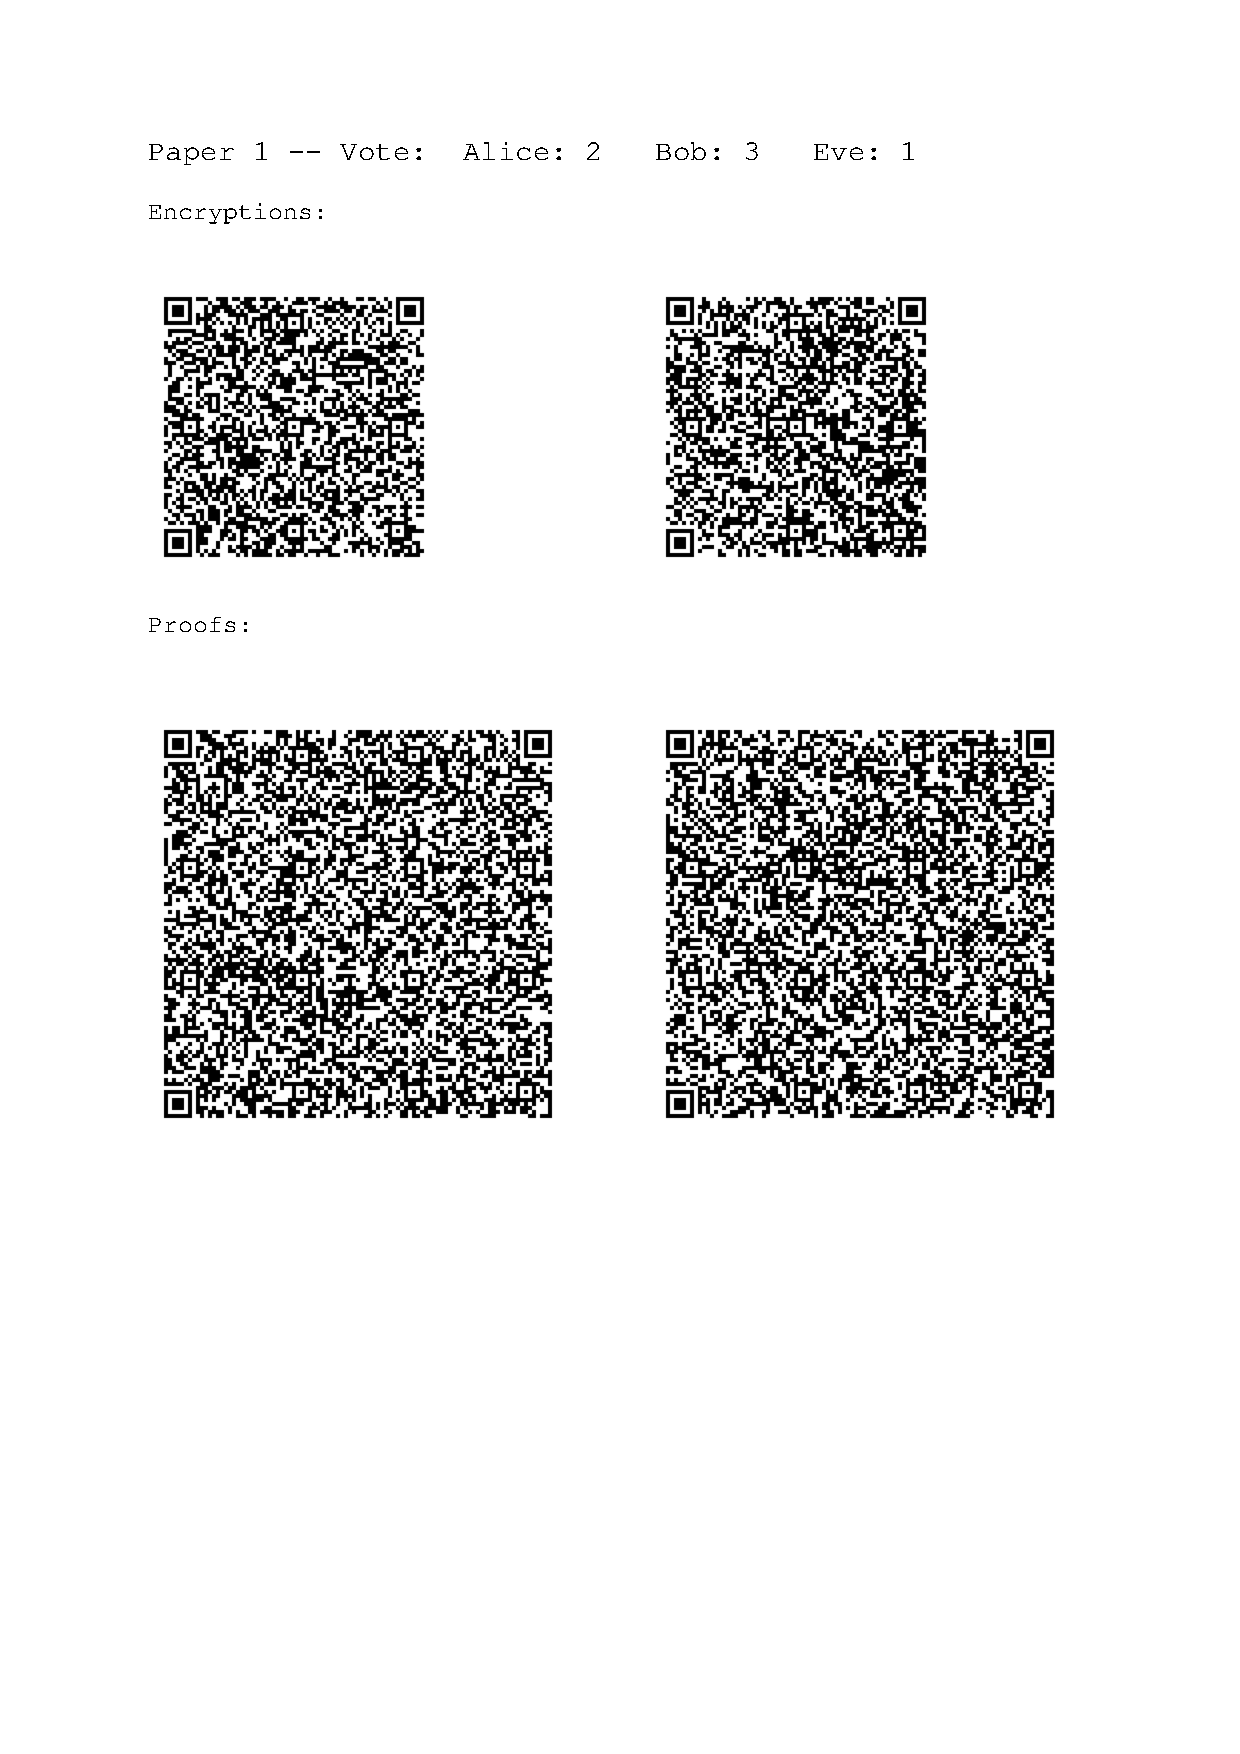
\includegraphics[scale=0.5, trim=2.5cm 10cm 3.1cm 0cm, clip=true]{paper1.pdf}
	\caption{Paper 1: The voter only needs to check the plaintext vote at the top.  This example illustrates a preferential vote: Eve first, Alice next and Bob last.}
	\label{fig:paper1}
\end{figure}

\begin{figure}
	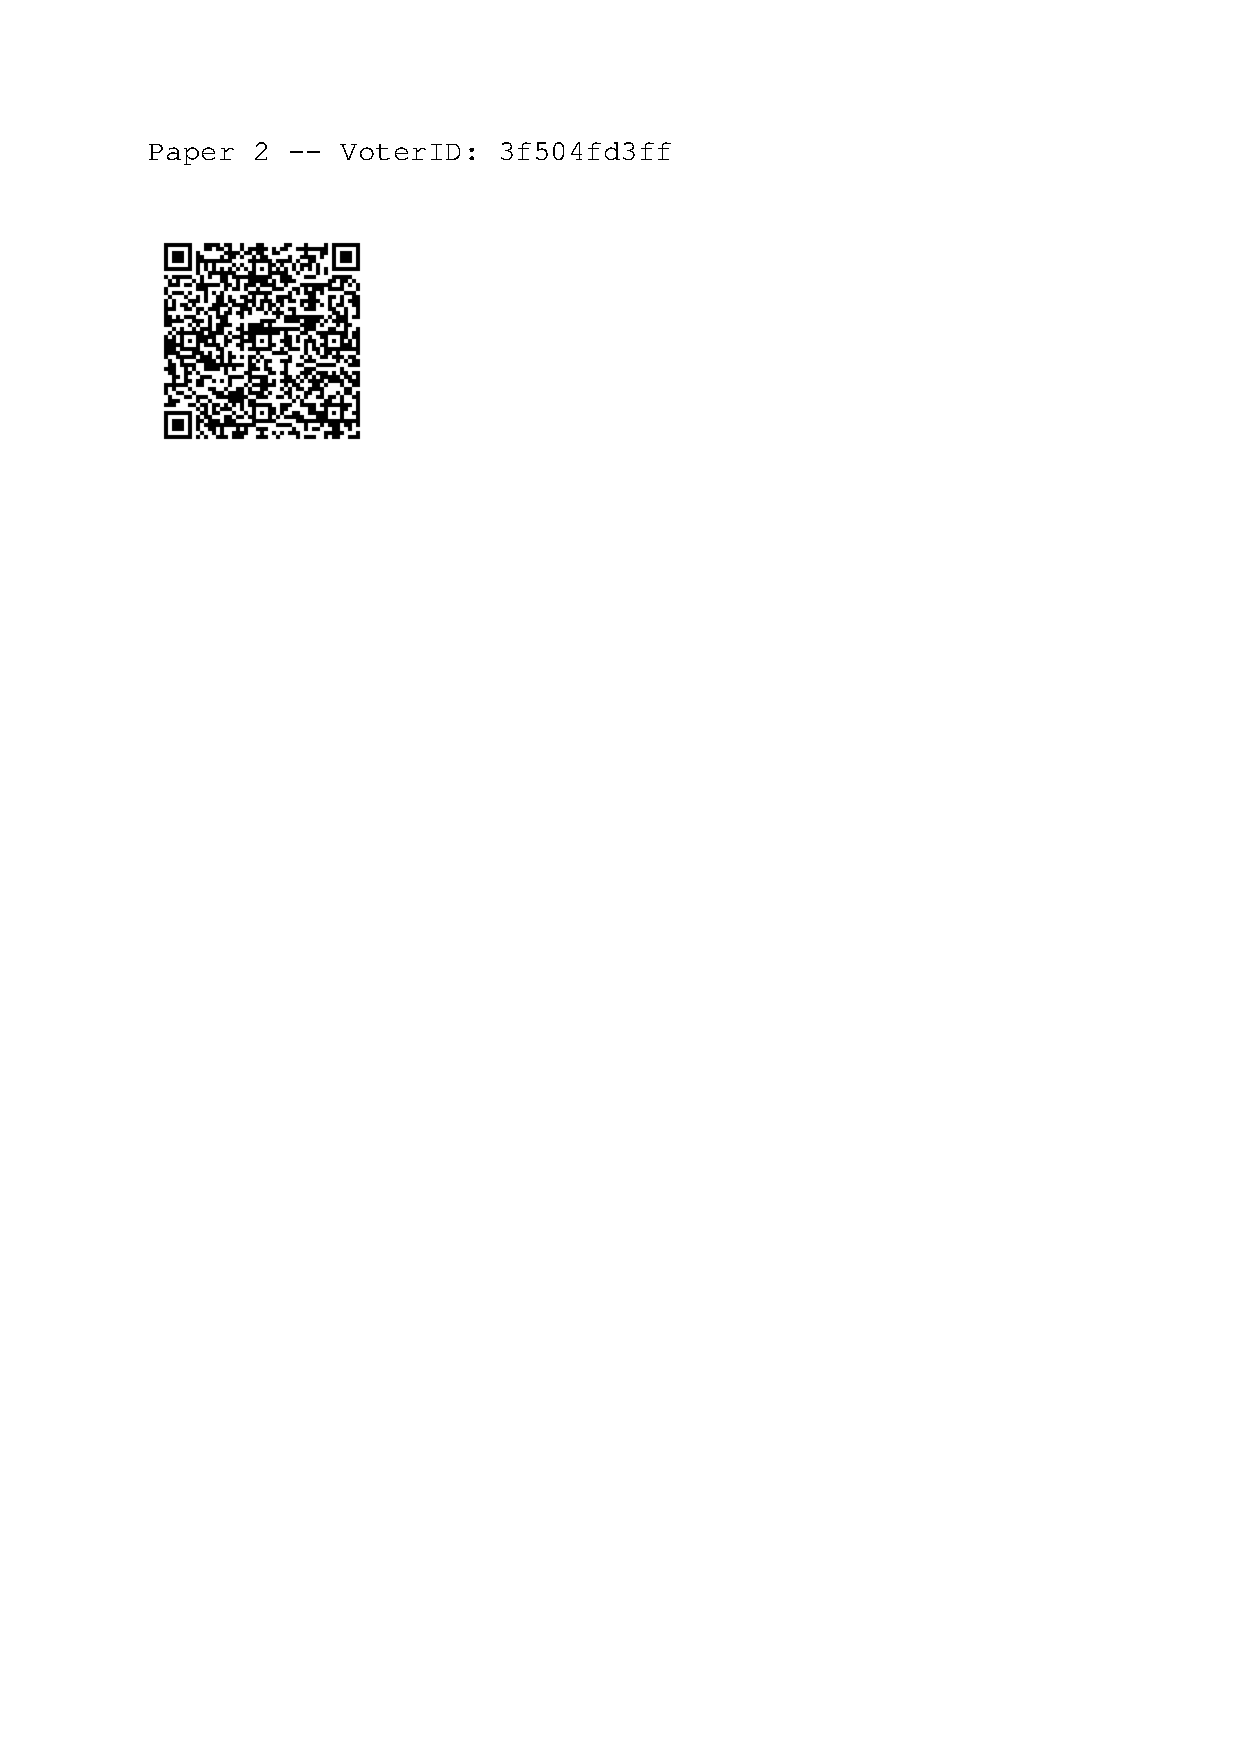
\includegraphics[scale=0.5, trim=0cm 22cm 4cm 0cm, clip=true]{paper2.pdf}
	\caption{Paper 2: The voter only needs to check the plaintext $\VoterID$.}
		\label{fig:paper2}
\end{figure}


\subsection{Tallying ballots}
Once the ballot casting period has ended, the electoral commission can begin receiving ballots. The voter ID as seen by the electoral commission is referred to as $\receivedvid$. First, the electoral commission checks the proof on Paper 2. 
They should also confirm that $\receivedvid$ matches the identification on the outside of the envelope. If it does, they should attach the encryption $\{\receivedvid\}_{pk}$ to Paper 1 (without opening it)\footnote{This could be done by e.g. tearing Paper 2 and stapling it to Paper 1, or even by providing $\{\receivedvid\}_{pk}$ on a third piece of paper.}, and destroy the rest of Paper 2. The set of Paper 1s from all ballots should now be shuffled physically, to preserve privacy.

After shuffling, the electoral commission receives Paper 1 as
$$\Paper_1=\left(ReceivedVote,\ \{a,b,r_a,r_b\}_{pk}, \PrfKnow(\{a,b,r_a,r_b\}_{pk}\right)$$
The electoral commission should check the proofs, and if they are valid, post the re-randomised received ballot to the WBB. This should be performed under scrutiny from e.g. party representatives to ensure they are faithfully posted; this is the only step that needs active scrutiny.

The electoral trustees next perform a cryptographic mix to produce a list of ballots of the form
$$\left(\{ReceivedVote\}_{pk},\ \receivedvid,\ (a,b,r_a,r_b)\right)$$
on the WBB. The resulting list should be joined to the commitments on the WBB by matching $ReceivedVoterID$ to $\VoterID$, producing a list of tuples
$$\left(\{ReceivedVote\}_{pk},\ \VoterID,\ (a,b,r_a,r_b), \commit(a;r_a), \commit(b;r_b)\right)$$
If there are multiple tuples for some $\VoterID$, for each tuple the pair of commitments $\commit(a;r_a)$, $\commit(b;r_b)$ should be checked. If the parameters $a,b,r_a,r_b$ are correct openings for exactly one tuple, only that tuple should be accepted; in any other case, no tuples for $\VoterID$ should be accepted.

The accepted tuples should then be matched with the electoral commission's commitments to produce a list of tuples
$$\left(\{\Vote\}_{pk},\{\Mac\}_{pk}, \{ReceivedVote\}_{pk},\ \VoterID,\ a, \{b\}_{pk}, \PrfEnc(b, \{b\}_{pk})\right)$$
For all accepted tuples, the electoral trustees should perform a plaintext equivalence test on the WBB to show whether $ReceivedVote=\Vote$ (without decrypting either). If this succeeds, using the homomorphic property of exponential ElGamal the electoral commission\footnote{This does not require the secret key, so it can be easily verified by any party.} constructs a second MAC from the received vote:
$$\{\Mac'\}_{pk}=a\cdot\{ReceivedVote\}_{pk}+\{b\}_{pk}$$
This is posted to the WBB with the voter ID and the committed vote-MAC pair:
$$\left(\VoterID, \{\Vote\}_{pk},\ \{\Mac\}_{pk},\ \{\Mac'\}_{pk}\right)$$
The electoral trustees perform another plaintext equivalence test on the WBB to show that $\Mac=\Mac'$. For all tuples that pass this test, the electoral trustees should decrypt $\{\Vote\}_{pk}$ to produce a final list of valid votes. (We assume that once the final list is public, someone counts the votes correctly.)

Note that anybody can check whether a given voter ID produced a valid vote by seeing whether a tuple $\left(\VoterID, \{\Vote\}_{pk},\ \{\Mac\}_{pk},\ \{\Mac'\}_{pk}\right)$ passed the final plaintext equivalence test, providing \textit{individual} verifiability. It is easy to modify the protocol to remove this property, instead providing \textit{group} verifiability; this may be desirable depending on the application.
\subsection{Verification procedure}
We provide a summary of the various checks that need to be performed to verify the election. Verification is broken into three separate domains. Each voter must check the paper printout herself, and whether her ID appears in the final mix. Scrutineers from third parties must observe the process of receiving paper ballots. Finally, the WBB transcript can in theory be verified by anyone; because this may not be a trivial computational task, we expect that trusted entities such as media organisations would perform verification of this transcript on voters' behalf.

One of the great challenges in paper elections is \textit{chain-of-custody}: once a paper ballot is filled out by a voter, it should never leave the sight of a trusted authority. Traditional postal voting breaks this requirement, as postal channels are demonstrably vulnerable to interception~\cite{stewart2010losing}. To address this issue, our protocol defines a weaker trust model than the traditional chain of custody. The protocol is verifiable as long as at least one of the below is honest:
\begin{itemize}
    \item the client's device
    \item the postal channel and the electoral commission
\end{itemize}
Thus an adversary can undetectably cheat in the election if they control both the device and the postal channel (and/or the electoral commission), but cannot win if they control only one. This seems a reasonable compromise, since if the electoral commission (or postal service) deliberately compromises voters' devices, this is indicative of systemic corruption that no cryptographic verification scheme can address.
\subsection{The algorithms}
We present a formal description of the procedures that define the protocol for reference.
\singlespacing
\begin{algorithm}
    \caption{\textit{Setup}$(\lambda)$\textit{:} System setup protocol}
	\begin{algorithmic}[1]
\LineComment{The following are posted to the WBB:}
\State $\langle \VoterID \rangle$, a list of IDs of eligible voters.  We assume that these are assigned one-on-one to each voter.
\State	$(G,H,P)$: the public parameters of a perfectly-hiding Pedersen Commitment scheme  generated such that nobody knows $\dlog_G H$, with security parameter $\lambda$.
\State $(\mathbb{G}, p, q, g, pk)$: the public parameters of the exponential ElGamal encryption scheme generated with security parameter $\lambda$.
(This is multiplicative-homomorphic $\bmod\ p$, or additively homomorphic $\bmod\ q$ if the message is in the exponent, where $q$ is the order of $g\bmod p$ in $\mathbb{G}$.)
\State  (The corresponding secret key  $sk$ is shared among the set of EC trustees $T$.)
\end{algorithmic}
	\label{alg:setup}
\end{algorithm}
\begin{algorithm}
    \caption{\textit{Cast:} Vote generation and casting protocol}
	\begin{algorithmic}[1]
	\State Device: $a,b,r_a,r_b\leftarrow_R\{1,\ldots,q-1\}$ (uniformly at random)
	\State Device: $c_a\leftarrow\commit(a;r_a), c_b\leftarrow\commit(b;r_b)$
	\State $Device\rightarrow \Wbb$: $\mathcal{B}^{ident}_i=(\VoterID, c_a, c_b)$\label{Step:VoterCommit}
	\State $Voter\rightarrow Device$: $\Vote$
	\State Device: $\Mac\leftarrow a\cdot Vote+b\bmod p$
	\State $Device\rightarrow EC$: $\VoterID, \{g^\Mac\}_{pk}, \{g^\Vote\}_{pk}, \PrfKnow(\{g^\Mac\}_{pk}), \PrfKnow(\{g^\Vote\}_{pk})$% \textit{proofs of knowledge}$
	\State $EC\rightarrow \Wbb$: $\mathcal{B}^{commit}_i=(\VoterID, \rerand\{g^\Mac\}_{pk}, \rerand\{g^\Vote\}_{pk})$ \label{Step:ECPostsVoteMAC}
	\State Device: Wait for $\VoterID$ to appear on WBB
	\State $Device\rightarrow \Paper_1$: $\Vote, \{a,b,r_a,r_b\}_{pk}, \PrfKnow(\{a,b,r_a,r_b\}_{pk})$
	\State $Device\rightarrow \Paper_2$: $\VoterID, \{\VoterID\}_{pk}, \PrfEnc(\VoterID, \{\VoterID\}_{pk})$
	\State $Voter\rightarrow EC$: $\Paper_1, \Paper_2$ (by paper mail)
	\end{algorithmic}
\label{alg:cast}
\end{algorithm}
\begin{algorithm}
    \caption{\textit{Tally:} Vote receiving and tallying protocol}
	\begin{algorithmic}[1]
	\For {$i$th ballot $(\Paper_1,\Paper_2)$ received via paper mail}
		\State $\Paper_2\rightarrow EC:\ \ \receivedvid,\{\receivedvid\}_{pk}, \PrfEnc(\receivedvid,\{\receivedvid\}_{pk})$
		\State EC: $\text{Checks }\receivedvid\text{ matches electoral roll}$
		\State EC: Verifies $\PrfEnc(\receivedvid,\{\receivedvid\}_{pk})$
		\State $\Paper_2\rightarrow\Paper_1:\ \{\receivedvid '\}_{pk}$\label{Step:AttachVID}
		\State $\qquad \qquad \qquad\text{Destroy }\Paper_2,\qquad\text{Shuffle }\Paper_1\downarrow$
		\State $\Paper_1\rightarrow EC:\ \ \ReceivedVote, \{\receivedvid\}_{pk},\{a,b, r_a, r_b\}_{pk},\PrfKnow(\{a,b, r_a, r_b\}_{pk})$
		\State EC: $\text{Verifies }\PrfKnow(\{a,b, r_a, r_b\}_{pk})$.\par
		\hskip\algorithmicindent On failure, skip ballot.
		\State $\textit{EC} \rightarrow \Wbb : \ \mathcal{B}^{\text{votes}}_i=(\ReceivedVote, \rerand\{\receivedvid\}_{pk},\rerand\{a,b, r_a, r_b\}_{pk})$    \label{Step:ECPostsPaperInfo}
	\EndFor
	\State $T\rightarrow \Wbb: \ \mathcal{B}^{\text{votes'}}=\Mix(\mathcal{B}^{\text{votes}})$\label{Step:MixCast}
	\For {$\mathcal{B}^{\text{votes'}}_i=(\{g^\ReceivedVote\}_{pk}, \{\receivedvid\}_{pk}, \{a,b, r_a, r_b\}_{pk})$}
		\State $T: (a, b, r_a, r_b) = \Dec(\{a,b,r_a,r_b\}_{pk})$\label{Step:DecryptParams}
		\State $T: \receivedvid = \Dec(\{\receivedvid\}_{pk})$\label{Step:DecryptID}
		\State $T\rightarrow \Wbb: \ \mathcal{B}^{\text{mixed}}_i=(\{g^\ReceivedVote\}_{pk}, (a,b, r_a, r_b), \receivedvid, \text{decryption proof})$ \label{Step:RecVoterIDToWBB}
	\EndFor
	\LineComment{Join by matching $\VoterID$ to $\receivedvid$}  \label{Step:FirstWBBMsgs}
	\For {$\mathcal{B}^{\text{mixed}}_i$ such that $\receivedvid$ is unique}
		%	\State Check that $a,b, r_a, r_b$ is a valid commitment opening of $c_a, c_b$   \& $\{MAC\}_{pk_1} $
		\For {$\mathcal{B}^{\text{ident}}_j=(\VoterID, c_a, c_b)$ such that $\VoterID=\receivedvid$}
			\If {$c_a=\commit(a;r_a)$ and $c_b=\commit(a;r_b)$}
				\State {mark $\mathcal{B}^{\text{ident}}_j$ as a correct commitment opening for $\mathcal{B}^{mixed}_i$}
			\EndIf
		\EndFor
		\If {exactly one $\mathcal{B}^{\text{ident}}_j$ is a correct opening for $\mathcal{B}^{\text{mixed}}_i$}
			
			% The below check ensures the EC didn't falsify the MAC commitment.
			% In particular, it's important we construct MAC' from the {Vote}_{pk} committed to by the EC.  
			\label{Step:uniqueCommitOpen}
			\State $\Wbb\rightarrow T:\ \mathcal{B}^{\text{commit}}_k=(\VoterID, \{g^\Vote\}_{pk}, \{g^\Mac\}_{pk})$\par
			\hspace{1cm}{If there is no $\mathcal{B}^{\text{commit}}_k$ with matching $\VoterID$, proceed to the next iteration.}
			\State $T\rightarrow \Wbb: \pet\big(\{g^\ReceivedVote\}_{pk}, \{g^\Vote\}_{pk}\big)$\label{Step:ECVotePEP}
			\State $\{g^{\Mac'}\}_{pk} := a \cdot \{g^\Vote\}_{pk} + \{g^b\}_{pk}$
			\State $T\rightarrow \Wbb: \pet\big(\{g^\Mac\}_{pk},\{g^{\Mac'}\}_{pk}\big)$\label{Step:ECMACPEP}
			\If{plaintext equivalence proofs pass}
				\State $T\rightarrow \Wbb:\ \mathcal{B}^{\text{accepted}}_i = \left(\VoterID, \{g^\Vote\}_{pk}\right)$\label{Step:PETsPassed}

			\EndIf
		\EndIf
	\EndFor
	\State $T\rightarrow \Wbb: \mathcal{B}^{accepted'}=\Mix(\mathcal{B}^{\text{accepted}})$\label{Step:MixAccepted}
	\LineComment{Produce final tally}
	\For {$\mathcal{B}^{\text{accepted'}}_i=\{g^\Vote\}_{pk}$ on $\Wbb$}
		\State $T\rightarrow \Wbb: \mathcal{B}^{\text{tally}}_i=\Dec(\{g^\Vote\}_{pk})$\label{Step:DecryptVote}
	\EndFor
	\end{algorithmic}
\label{fig:tally}
\end{algorithm}
\onehalfspacing
\newpage
\section{Properties and trust assumptions}\label{sec-properties}
The standard approach to proving desirable properties of cryptographic protocols is to define a \textit{game} between an adversary and a challenger, and to argue that the adversary can win only if they are very lucky. This is made formal below.
\begin{definition}[Negligible function]
    A function $f:\mathbb{N}\rightarrow\mathbb{R}$ is \textit{negligible} if for all polynomials $\poly(x)$, there exists $N>0$ such that for all $x>N$

    $$|f(x)|<\frac{1}{\poly(x)}$$

    We will write $\Pr[A]=\negl(\lambda)$ as shorthand to mean ``there exists a negligible function $\negl$ such that $\Pr[A]=\negl(\lambda)$''.
\end{definition}
Our adversary then should only be able to win the game with a negligible probability as a function of some security parameter. To formally define what we mean by ``adversary'':
\begin{definition}[Probabilistic polynomial-time (PPT) adversary]
    A \textit{probabilistic polynomial-time adversary} (denoted $\mathcal{A}$) is an algorithm (typically interactive) that runs in polynomial time and has access to a randomness source.
\end{definition}
Many of the games we will use involve the adversary choosing a bit; it follows that the adversary can always win with at least 50\% probability, so we will instead talk about a negligible \textit{advantage} over tossing a coin. 
\begin{definition}[Advantage]
    An adversary $\mathcal{A}$ has \textit{advantage} $\varepsilon$ in game $G$ if
    $$\Pr\left[\mathcal{A}\text{ wins }G\right]=\varepsilon$$
    We will write $\Adv(\mathcal{A}, G)=\varepsilon$.

    Given two games $G_i, G_j$, we say $\mathcal{A}$'s \textit{advantage between} the two games is
    $$\Adv_{G_i, G_j}(\mathcal{A}) = \frac{1}{2}
    \Big|
        \Adv(\mathcal{A}, G_i)
         -
        \Adv(\mathcal{A}, G_j)
    \Big|$$
\end{definition}
\subsection{Privacy}
Any practical voting scheme needs to guarantee the privacy of its voters. To be more precise, it should ideally not be possible for anybody to determine which vote was cast by a particular voter except the voter themselves. Postal voting demands that voters' identities be verified on receipt of the vote; this means that the electoral commission could in principle break a voter's privacy. However, real-world postal voting systems have steps in place to preserve voters' privacy. For example, in Australian elections voters' identities are checked by having the voter write their name and address on the envelope, and fold their ballot before placing it inside. In this way, the voter's identity can be verified, then the envelope can be opened and the still-folded ballot can be passed to somebody who did not learn the voter's identity. Our protocol involves a similar procedure. Privacy is distinct from \textit{receipt freeness}, which demands that a voter not be able to prove which vote they cast to anybody else.

Our definition of privacy is based on that of~\cite{kiayias2015end}. We separate voter privacy from receipt freeness because we can prove privacy against a stronger adversary than for receipt freeness. For privacy, we will remove the simulator defined by~\cite{kiayias2015end}---the purpose of the simulator is to allow a voter to lie about their vote, which is not relevant in the privacy-only case.

Voter privacy is defined as a game between a PPT adversary $\mathcal{A}$ and a challenger $\mathcal{C}$. We consider a set of $m$ candidates $\mathcal{P}=\{P_1,\ldots,P_m\}$, a set of $n$ voters $\mathcal{V}=\{V_1,\ldots,V_n\}$, a set of allowed candidate selections $\mathcal{U}$ (which may be a single choice, or a numbered preference list, or whatever is appropriate) and an \textit{election evaluation function} $f(\langle \mathcal{U}_1,\ldots,\mathcal{U}_n \rangle)$ mapping the voters' candidate selections to a vector where the $i$th index contains the number of votes for candidate $\mathcal{P}_i$. The general idea is that the adversary chooses the parameters for the election and may choose to \textit{corrupt} a number of voters of its choice, meaning that it acts as the voter. The challenger acts as the EC, WBB, and election trustees, and acts on behalf of honest voters; for each non-corrupted voter, the adversary provides the challenger with two votes to choose from. The adversary wins if it is able to guess which of the two votes the non-corrupted voters cast \textbf{and} the adversary did not choose the parameters so that it always wins. An in-depth discussion of this second condition follows the formal definition below.

\begin{definition}[Voter privacy]
    Consider the below game between an adversary $\mathcal{A}$ and a challenger $\mathcal{C}$, written $G^\mathcal{A}_{\text{Privacy}}(1^\lambda, n, m)$.
    \begin{enumerate}
        \item Given $1^\lambda, n, m$, $\mathcal{A}$ chooses a set of candidates $\mathcal{P}=\{P_1,\ldots,P_m\}$, voters $\mathcal{V}=\{V_1,\ldots,V_n\}$, and candidate selections $\mathcal{U}$. It sends the sets $\mathcal{P}, \mathcal{V},$ and $\mathcal{U}$ to $\mathcal{C}$.
        \item $\mathcal{C}$ tosses a coin $b\in\{0, 1\}$, and runs the $\mathsf{Setup}$ protocol to obtain parameters for ElGamal encryption and Pedersen commitment. It sends the public parameters to $\mathcal{A}$.
        \item $\mathcal{A}$ schedules the $\mathit{Cast}$ protocol for all voters, which are allowed to run concurrently. For all $V_l\in\mathcal{V}$, the adversary chooses whether $V_l$ is to be corrupt.
        \begin{itemize}
            \item If $V_l$ is corrupt, $\mathcal{A}$ acts on $V_l$'s behalf as it wishes.
            \item If $V_l$ is honest, $\mathcal{A}$ sends two candidate selections $\mathcal{U}_l^0, \mathcal{U}_l^1$ to $\mathcal{C}$. It must do so such that $f(\langle\mathcal{U}_l^0\rangle_{V_l\in \tilde{\mathcal{V}}})=f(\langle\mathcal{U}^1_l)_{V_l\in \tilde{\mathcal{V}}}\rangle`$ where $\tilde{\mathcal{V}}$ is the set of honest voters (that is, the set of honest votes alone does not leak $b$). $\mathcal{C}$ acts on $V_l$'s behalf to cast the vote $\mathcal{U}_l^b$. During this process $\mathcal{A}$ may view the encrypted data $\{\Vote\}_{\mathit{pk}}, \{\Mac\}_{\mathit{pk}}$ in transit to the EC, as well as the WBB and $\Paper_1, \Paper_2$ (after shuffling).
        \end{itemize}
        \item $\mathcal{C}$ runs the $\mathit{Tally}$ protocol, acting as the EC, the trustee set $T$, and the WBB. $\mathcal{A}$ may continue to observe the WBB.
        \item $\mathcal{A}$ outputs a bit $b^*$.
    \end{enumerate}
    $\mathcal{A}$ wins the game if and only if $b=b^*$. A scheme achieves \textit{voter privacy} if for all PPT adversaries $\mathcal{A}$, $\Adv\left(G^\mathcal{A}_{\text{Privacy}}(1^\lambda, n, m)\right)=\negl(\lambda)$.
\end{definition}
This definition contains some very careful phrasing. Note first what the adversary is allowed to learn: it can see anything on the WBB, anything on $\Paper_2$ for all voters, anything on $\Paper_1$ for all voters (but \textbf{not} which $\Paper_2$ corresponds to it for honest voters), and any of the encrypted data sent to the EC (but \textbf{not} an honest voter's view of how it was constructed). This is more general than what we will allow for receipt-freeness.

It is worth discussing some details in the condition placed on the adversary's choice of candidate selections in step 3. This prevents any attempt by the adversary to trivialise the problem by forcing the election's outcome alone to reveal $b$, and in particular prevents the adversary choosing all but one voter to be corrupt---since the list of decrypted votes on the WBB would reveal the cast vote. This is important since the protocol reveals not only the winner of the election, but also a full list of all valid votes.

A proof that our scheme satisfies this property follows. The goal will be to sequentially alter the privacy game, where each step is negligibly distinguishable from the previous step so that the adversary does not notice the manipulations. We will arrive at a game where none of the ciphertexts contain any information, so the adversary has no hope of winning.

\begin{theorem}\label{thm-privacy}
    For all constants $m \in \mathbb{N}$ and $n=poly(\lambda)$, the voting system described in Section~\ref{sec-protocol} satisfies voter privacy.
\end{theorem}
\begin{proof}
    We will use a hybrid argument to construct a sequence of games until we arrive at one in which the adversary clearly cannot have any advantage.
    \begin{itemize}[leftmargin=4em]
        \item[Game] $G_0$: the unaltered game $G^\mathcal{A}_{\text{Privacy}}(1^\lambda, n, m)$. By definition $\Adv_{G_0, G^\mathcal{A}_{\text{Privacy}}(1^\lambda, n, m)}(\mathcal{A})=0$.
        
        \item[Game] $G_1$: the same as Game $G_0$, except the decryption and plaintext equivalence tests on the WBB are generated using knowledge of their plaintexts; this is possible since every ciphertext is either generated by the challenger, or is generated by the adversary with an accompanying ZKP proving knowledge (so the challenger can use the corresponding zero-knowledge extractor). The soundness error in the adversary's ZKPs gives $\Adv_{G_1, G_0}(\mathcal{A})=\negl(\lambda)$.
 
        \item[Game] $G_2$: the same as Game $G_1$, except the ZKPs used to prove correctness of the decryptions and PETs are simulated via the zero-knowledge simulator. The ZKPs are non-malleable and the WBB filters for duplicates, so the adversary's proofs cannot depend on the simulated proofs---we are therefore still able to use the extractor from Game $G_1$. Note that the challenger no longer uses the ElGamal secret key for any purpose. The simulator has no error, so $\Adv_{G_2, G_1}(\mathcal{A})=0$.
 
        \item[Game] $G_3$: the same as Game $G_2$, except the mixing proofs are also simulated via the zero-knowledge simulator to ensure no information about the permutation or randomness used is leaked. As in $G_2$, we have $\Adv_{G_3, G_2}(\mathcal{A})=0$.
        
        \item[Game] $G_4$: the same as Game $G_3$, except the ciphertexts are replaced with encryptions of random values from an oracle (and re-randomisations are replaced with fresh encryptions of random values). No ciphertexts are ever decrypted,\footnote{If we did decrypt ciphertexts, the adversary could learn the decryptions of certain ciphertexts and use this to undermine the IND-CPA property.} so we can use the IND-CPA property of ElGamal to guarantee that $\Adv_{G_4,G_3}(\mathcal{A})=\negl(\lambda)$ (because the adversary cannot tell the ciphertexts were replaced).
    \end{itemize}
    In Game $G_4$, the encryptions are random and contain no usable information, and the link between $\VoterID$ and $\Vote$ is destroyed by the mix, so the adversary cannot have any advantage in guessing which vote was cast by each voter. Therefore, $\Adv(\mathcal{A}, G_3)=0$, which implies $\Adv\left(G^\mathcal{A}_{\text{Privacy}}(1^\lambda, n, m)\right)=\negl(\lambda)$ as required.
\end{proof}
\subsection{Receipt-freeness}
The game used for receipt-freeness will be similar to the privacy game, with two key differences:
\begin{enumerate}
    \item The adversary's view is restricted to the WBB and the view of the voter's client (\textbf{not} the pieces of paper).
    \item The voter has access to a simulator algorithm $\mathcal{S}$ that can \textit{simulate} their client's view to support a claim that they submitted a different vote.
\end{enumerate}

The goal will be to demonstrate that a voter can present a convincing argument that they submitted a vote that does not match the vote they sent in the mail. This protects the voter from coercion, but also prevents the voter selling her vote, as a buyer cannot tell whether or not the voter is being honest. We demonstrate this property for an honest-but-curious voter (i.e. one who does not actively deviate from the protocol), and we do not prove ``over-the-shoulder'' coercion-resistance: an adversary who watches the voter seal and post her envelope can be certain how she voted. A formal definition follows.
\begin{definition}[Receipt-freeness]
    Consider the below game between an adversary $\mathcal{A}$ and a challenger $\mathcal{C}$, written $G_{\text{Rec-free}}^{\mathcal{A},\mathcal{S}}(1^\lambda, n, m)$.
    \begin{enumerate}
        \item Given $1^\lambda, n, m$, $\mathcal{A}$ chooses a set of candidates $\mathcal{P}=\{P_1,\ldots,P_m\}$, voters $\mathcal{V}=\{V_1,\ldots,V_n\}$, and candidate selections $\mathcal{U}$. It sends the sets $\mathcal{P}, \mathcal{V},$ and $\mathcal{U}$ to $\mathcal{C}$.
        \item $\mathcal{C}$ tosses a coin $b\in\{0, 1\}$, and runs the $\mathsf{Setup}$ protocol to obtain parameters for ElGamal encryption and Pedersen commitment. It sends the public parameters to $\mathcal{A}$.
        \item $\mathcal{A}$ schedules the $\mathit{Cast}$ protocol for all voters, which are allowed to run concurrently. For all $V_l\in\mathcal{V}$, the adversary chooses whether $V_l$ is to be \textit{corrupt} or \textit{honest}.
        \begin{itemize}
            \item If $V_l$ is corrupt, $\mathcal{A}$ acts on $V_l$'s behalf as it wishes.
            \item If $V_l$ is honest, $\mathcal{A}$ sends two candidate selections $\mathcal{U}_l^0, \mathcal{U}_l^1$ to $\mathcal{C}$. It must do so such that $f(\langle\mathcal{U}_l^0\rangle_{V_l\in \tilde{\mathcal{V}}})=f(\langle\mathcal{U}^1_l)_{V_l\in \tilde{\mathcal{V}}}\rangle`$ where $\tilde{\mathcal{V}}$ is the set of honest voters (that is, the set of honest votes alone does not leak $b$). $\mathcal{C}$ acts on $V_l$'s behalf to cast the vote $\mathcal{U}_l^b$. During this process $\mathcal{A}$ may view \textbf{only} the WBB. After $\mathit{Cast}$ terminates, $\mathcal{C}$ provides to $\mathcal{A}$:
            \begin{enumerate}
                \item the \textit{receipt} $\alpha_l$ consisting of voter $V_l$'s $\VoterID$
                \item if $b=0$, $V_l$'s real view (including randomness for the encryptions)
                \begin{gather*}
                    a, b, r_a, r_b, \Vote=\mathcal{U}^0_l, \Mac,\\\{g^\Vote\}_{pk}, \{g^\Mac\}_{pk}, \{a,b,r_a,r_b\}_{pk},\{\VoterID\}_{pk}
                \end{gather*}
                If $b=1$, $\mathcal{C}$ instead provides a simulated view using $\mathcal{S}$.
            \end{enumerate}
        \end{itemize}
        \item $\mathcal{C}$ runs the $\mathit{Tally}$ protocol, acting as the EC, the trustee set $T$, and the WBB. $\mathcal{A}$ may continue to observe the WBB.
        \item $\mathcal{A}$ outputs a bit $b^*$.
    \end{enumerate}
    $\mathcal{A}$ wins the game if and only if $b=b^*$. A scheme achieves \textit{receipt freeness} if there exists a simulator $\mathcal{S}$ such that for all PPT adversaries $\mathcal{A}$, $\Adv\left(\mathcal{A}, G^{\mathcal{A},\mathcal{S}}_{\text{Rec-free}}(1^\lambda, n, m)\right)=\negl(\lambda)$.
\end{definition}

We will prove this property by having the electoral commission secretly swap the coerced voters' encrypted data so that the mixing and decryption falsely proves they obeyed the adversary, and argue that an adversary cannot tell the difference. The voter $V_l$ will be asked to vote according to the selection $\mathcal{U}^0_l$, but will actually vote according to $\mathcal{U}^1_l$. She will tell the truth about her secrets $a, b, r_a, r_b$, but will claim to have sent the MAC $a\cdot\mathcal{U}^0_l+b$ instead of the MAC corresponding to her vote. The adversary cannot watch the electoral commission randomising the MAC, so cannot tell the difference. Swapping the encrypted data received in the post will allow the EC to prove plaintext equivalence of the encrypted data and the claimed vote.
\begin{theorem}\label{thm-Rec-free}
    For all constants $m \in \mathbb{N}$ and $n=poly(\lambda)$, the voting system described in Section~\ref{sec-protocol} satisfies receipt freeness.
\end{theorem}
\begin{proof}
    First, we define the simulator. $\mathcal{S}$ receives an honest voter's view
    \begin{gather*}
        a, b, r_a, r_b, \Vote=\mathcal{U}^1_l, \Mac,\\\{g^\Vote\}_{pk}, \{g^\Mac\}_{pk}, \{a,b,r_a,r_b\}_{pk},\{\VoterID\}_{pk}
    \end{gather*}
    It computes a valid MAC for the claimed vote $\mathcal{U}^0_l$ as well as ciphertexts for the claimed vote and MAC. It then outputs the simulated view
    \begin{gather*}
        a, b, r_a, r_b, \Vote'=\mathcal{U}^0_l, \Mac'=a\cdot\Vote'+b\,\\\{g^{\Vote'}\}_{pk}, \{g^{\Mac'}\}_{pk}, \{a,b,r_a,r_b\}_{pk},\{\VoterID\}_{pk}
    \end{gather*}

    We will use a hybrid argument to prove the result as per Theorem~\ref{thm-privacy}.
    \begin{itemize}[leftmargin=4em]
        \item[Game] $G_0$: The actual game $G^{\mathcal{A},\mathcal{S}}_\text{Rec-free}(1^\lambda,n,m)$, where the challenger uses $\mathcal{U}^b_l$ in the $\mathit{Cast}$ protocol and the above simulator is invoked when $b=1$.  (That is, voters vote as they wish and run the coercion-resistance strategy.)
        
        By definition $\Adv_{G_0,G^{\mathcal{A},\mathcal{S}}_{\text{Rec-free}}(1^\lambda,n,m)}(\mathcal{A}) = 0$.
    
        \item[Game] $G_1$: The same as Game $G_0$, except the decryptions and plaintext equivalence tests are simulated with knowledge of the plaintext as in Theorem~\ref{thm-privacy}; $\Adv_{G_1, G_0}(\mathcal{A})=\negl(\lambda)$.
    
        \item[Game] $G_2$: The same as Game $G_1$, except the proofs used to demonstrate correct decryption and plaintext equivalence are simulated with their zero-knowledge simulators as in Theorem~\ref{thm-privacy}. We then have $\Adv_{G_2, G_1}(\mathcal{A})=0$.
 
        \item[Game] $G_3$: The same as Game $G_2$, except the proof of correct mixing is simulated as in Theorem~\ref{thm-privacy}. To ensure the link between successive ciphertexts is destroyed, the challenger uses knowledge of the plaintext to replace ciphertexts with fresh encryptions after each mix. We have $\Adv_{G_3, G_2}(\mathcal{A})=0$.
    
        \item[Game] $G_4$: The same as Game $G_3$, except when $b = 1$:
        \begin{enumerate}
            \item In Step ? of $\mathit{Cast}$, the challenger posts an encryption of the claimed MAC, $\{g^{\Mac'}\}_{pk}$, instead of a re-randomised encryption of the actual MAC $\{g^\Mac\}_{pk}$.
            \item In Step ? of $\mathit{Tally}$, the challenger changes the posted (re-randomised) encryptions of $\receivedvid$ and $a, b, r_a, r_b$ so that they appear together with the votes they claimed to have cast.
        \end{enumerate}
        $\mathit{Tally}$ can then proceed as usual; we have changed the votes and MACs consistently so that they are still plaintext-equivalent. Since all we have done is change encryptions for which the adversary does not know the randomness and the link between successive ciphertexts is destroyed, the IND-CPA property of ElGamal yields $\Adv_{G_4, G_3}(\mathcal{A})=\negl(\lambda)$.
    
        \item[Game] $G_5$: The same as Game $G_4$, except the challenger (acting as the honest voters) ignores the value of $b$ and always obeys the adversary. Since the adversary does not see anything different to what it saw in Game $G_4$, $\Adv_{G_5, G_4}(\mathcal{A})=0$.
    \end{itemize}
    The adversary can have no advantage in Game $G_5$ because the value of $b$ is ignored. Following the chain of games then yields
        $$\Adv_{G_5, G^{\mathcal{A},\mathcal{S}}_\text{Rec-free}(1^\lambda,n,m)}=negl(\lambda)$$
    as required.
\end{proof}
\subsection{Verifiability}
A major benefit that cryptographic voting brings is \textit{verifiability:} it is possible to provide the public with a degree of evidence that the election was carried out correctly. In traditional paper elections, it is common to request officials known as \textit{scrutineers} from each party to observe the vote counting process and ensure its impartiality. This is distinct from public information that can give some confidence of correctness to everybody, not just those present when the votes are being counted.

The holy grail of verifiability is \textit{universal verifiability}, which demands that any observer may be confident of the election's correctness even assuming every stage of the process is corrupted. Our protocol \textbf{does not} satisfy this strong requirement---we settle for a weaker version where the election is verifiable assuming \textbf{either} the voter's client is honest, \textbf{or} the electoral commission (including the paper channel) is honest.

% TODO: comment on scrutineers. They help prevent denial of service, but the EC can't get away with cheating even if they're colluding with scrutineers.
%We also rely on scrutineers to ensure paper ballots are faithfully recorded on the web bulletin board.

For more detail on the distinctions between verifiable elections and \textit{universally} verifiable elections, as well as a demonstration of how these distinctions can go wrong, see .
% TODO: cite myself

\subsubsection{With a cheating EC}
To prove that a cheating electoral commission will be caught during verification (assuming an honest client), we will argue that it must post a valid MAC for the wrong vote, and therefore that it must know the targeted client's secrets $a$ and $b$. After the election, the WBB contains three lists:
\begin{enumerate}
    \item a list of registered voters---those who have uploaded a valid VoterID and commitments
    \item a list of plaintext ballots posted by the EC during $\mathit{Tally}$
    \item a mixed list of the votes from ballots that uniquely matched a registered voter's commitments and passed the plaintext equality tests
\end{enumerate}
Clearly if List 3 is not a subset of List 2, something has gone wrong---an extra ballot has appeared from nowhere. This can only happen by breaking the soundness of the mix or the decryption proofs, so happens with only negligible probability.

However in a normal election (with no cheating) there will be some rows that go missing between Lists 1 and 3: some voters may register but not vote, some votes may be lost in the mail, and some votes may be incorrectly recorded on arrival. We would like to define what an \textit{acceptable} election outcome is, where fraud will be detected but a small discrepancy will not cause the whole election to fail. The votes in List 3 are those for which everything worked out perfectly and no fraud was detected. Votes that go missing between Lists 1 and 3 could be due to aforementioned errors, or they could indicate possible fraud. A few examples:
\begin{itemize}
    \item ballots may have been intercepted and either destroyed (causing the ballot to be missing from List 2) or modified (causing the vote to be missing from List 3)
    \item voters' devices could have been compromised by malware (causing the ballot to be rejected on arrival and thus be missing from List 2, or to fail verification and be missing from List 3)
    \item votes could have been intentionally dropped by the electoral commission and be missing from List 3
\end{itemize}

In summary, List 3 gives a claimed election outcome while Lists 1 \& 2 provide some evidence for errors and attempted fraud. Let $\mathcal{O}$ be the outcome of the election (e.g. a map from candidates to vote counts) with margin $M$ according to the paper record (e.g. the difference in vote counts between the top two candidates), and $0 \leq d < M$ be the acceptable number of caught errors according to the WBB transcript. One obvious formula would be: accept the election outcome $\mathcal{O}$ if the plaintext ballots give the same winner as List 3 (i.e. $d = M - 1$).  Another possible rule would be: accept $\mathcal{O}$ if the margin is greater than
$d = |\text{List 3}| - |\text{List 2}|$ 
plus the number of voter IDs with duplicate matches in Step~\ref{Step:uniqueCommitOpen} of \textit{Tally}; this would capture the idea that the election margin was greater than the amount of demonstrated error or fraud.

We define the result from the WBB transcript $\tau$:
$$\mathbf{Result}(\tau)=
\begin{cases}
    f(\mathcal{O})  &   \text{if the error according to }\tau\text{ is less than }\delta\\
    \bot            &   \text{otherwise}
\end{cases}$$
To compare the margin to the threshold, we will use a \textit{metric} $d(\cdot,\cdot)$. For example, in first-past-the-post elections where $\mathcal{O}$ counts the number of votes for each candidate, this could be the Manhattan metric
$$d_1(a, b)=\sum_{i=1}^n |a_i-b_i|$$

Our definition of verifiability will again be based on that from \cite{kiayias2015end}, modified so that the adversary cannot control both the EC and the voter's client at the same time. Since the adversary is not required to ever properly cast a vote, we will use a \textit{vote extractor} algorithm $\mathcal{E}\left(\tau, \langle \alpha_l \rangle\right)$ which extracts the dishonest votes $\langle \mathcal{U}_l \rangle_{\mathcal{V}_l\in\mathcal{V}\setminus\tilde{\mathcal{V}}}$ from the transcript $\tau$ and honest voters' receipts $\langle \alpha_l \rangle$\footnote{Recall these are simply the VoterIDs.}, possibly in super-polynomial time. In our protocol there is no situation where the adversary casts an invalid vote---such attempts instead contribute zero to the vote count. The extractor exists instead to capture the fact that we do not immediately assume a well-behaved adversary.

We will also require that a threshold of honest voters $\theta$ successfully cast their vote. A formal definition follows. Note unlike the previous games, in this game the \textit{adversary} controls the encryption parameters.

\begin{definition}[EC Verifiability]
    Consider the below game between an adversary $\mathcal{A}$ and a challenger $\mathcal{C}$, written $G_\text{EC-ver}^{\mathcal{A},\mathcal{E},\delta,d,\theta}(1^\lambda, m, n)$.
    \begin{enumerate}
        \item Given $1^\lambda, n, m$, $\mathcal{A}$ chooses a set of candidates $\mathcal{P}=\{P_1,\ldots,P_m\}$, voters $\mathcal{V}=\{V_1,\ldots,V_n\}$, and candidate selections $\mathcal{U}$. $\mathcal{A}$ runs the $\mathsf{Setup}$ protocol to obtain parameters for ElGamal encryption and Pedersen commitment. It sends the public parameters and the sets $\mathcal{P}, \mathcal{V}, \mathcal{U}$ to $\mathcal{C}$.
        
        \item $\mathcal{A}$ schedules the $\mathit{Cast}$ protocol for all voters, which are allowed to run concurrently. For all $V_l\in\mathcal{V}$, $\mathcal{A}$ chooses whether $V_l$ is to be \textit{corrupt} or \textit{honest}.
        \begin{itemize}
            \item If $V_l$ is corrupt, $\mathcal{A}$ acts on $V_l$'s behalf as it wishes.
            \item If $V_l$ is honest, $\mathcal{A}$ sends a candidate selection $\mathcal{U}_l$ to $\mathcal{C}$, which acts on $V_l$'s behalf to cast the vote $\mathcal{U}_l$.
        \end{itemize}

        \item $\mathcal{C}$ engages with $\mathcal{A}$ in the $\mathit{Cast}$ protocol so that $\mathcal{A}$ acts as the electoral commission and the postal service. For each voter $V_l$, $\mathcal{C}$ receives the receipt $\alpha_l=\VoterID$.

        \item $\mathcal{A}$ posts the election transcript $\tau$ to the WBB.
    \end{enumerate}
    Let $\tilde{\mathcal{V}}$ be the set of successfully-verifying honest voters. $\mathcal{A}$ wins the game if and only if:
    \begin{enumerate}
        \item $|\tilde{\mathcal{V}}| \geq \theta$ (i.e. at least $\theta$ honest voters verified successfully);
        \item $\forall l \in [n]:$ if $V_l \in \tilde{\mathcal{V}}$, then Verify$(\tau, \alpha_l) 	=1$ (i.e. the voters in $\tilde{\mathcal{V}}$ verify their votes successfully);
    
        \item $\mathbf{Result}(\tau) \neq \bot$; and
        \item for the metric $d(\cdot, \cdot)$ and election outcome function $f$:
                    $$d(\mathbf{Result}(\tau), f(\langle\mathcal{U}_1,\ldots,\mathcal{U}_n\rangle)) \geq \delta$$
            where $\{\mathcal{U}_l\}_{V_l \in \mathcal{V} \setminus \tilde{\mathcal{V}}} \leftarrow \mathcal{E}(\tau, \{\alpha_l \}_{V_l \in \tilde{\mathcal{V}}})$
            (That is, the deviation from the true result is larger than the accepted deviation $d$.)
    \end{enumerate}
    A scheme achieves \textit{EC verifiability} if for all PPT adversaries $\mathcal{A}$, $$\Pr\left[\mathcal{A}\text{ wins }G_\text{EC-ver}^{\mathcal{A},\mathcal{E},\delta,d,\theta}\right]=\negl(\lambda)$$
\end{definition}
The proof will proceed by considering a simplified version of the protocol in which there is only one trustee holding the decryption key (since we have already proved privacy). The adversary can easily drop a vote whenever they want; we are interested in the case where they accept a vote, but try to change what it says.

\begin{theorem}
    For any constant $m\in\mathbb{N}$ and $n=poly(\lambda)$, a specified result function $\mathbf{Result}(\tau)$ defining a threshold $0 \leq d < M$ for an election with margin $M$, and $\theta=|\mathcal{V}|-(M-d)$, the simplified ZKP-based version of the protocol satisfies EC verifiability.
\end{theorem}
\begin{proof}
    We begin by defining the vote extractor $\mathcal{E}$. For each corrupt voter ID, it considers the commitment pair posted by the voter's device in Step~\ref{Step:VoterCommit} of Algorithm~\ref{fig:genAndCasting}, and the encrypted vote-MAC pair posted by the EC in Step~\ref{Step:ECPostsVoteMAC} of Algorithm~\ref{fig:genAndCasting}. It inspects the WBB transcript $\tau$ and outputs:
    \begin{enumerate}
        \item zero, if the voter ID has no matches in Step~\ref{Step:FirstWBBMsgs} of Algorithm~\ref{fig:tallying} or no correct opening is seen in Step~\ref{Step:uniqueCommitOpen} of Algorithm~\ref{fig:tallying}
        \item zero, if the voter ID has more than one such match and correct opening
        \item zero, if there is a unique match and correct opening but either of the PETs and/or associated proofs in Steps~\ref{Step:ECVotePEP} and~\ref{Step:ECMACPEP} are not successful
        \item $\ReceivedVote$ otherwise
    \end{enumerate}

    The first three cases correspond to a vote that was not submitted, or a verification failure. Case 4 represents successful verification of a vote that makes it into the tally. We will argue that the adversary has a small probability of successfully (and undetectably) substituting a vote with a different one in this case; we therefore allow a small deviation $\delta$ from the correct result. If the adversary can forge any of the zero-knowledge proofs, they have the ability to do this substitution; for example, a forged mix proof could allow the output list to not match its input list, or a forged decryption proof could make a false claim about an encrypted vote. The soundness properties for these proofs guarantee the adversary has a negligible probability $\eta=\negl(\lambda)$ of doing so successfully.

    From here we assume the zero-knowledge proofs are true; that is, the statement they assert is true, and there is some witness for each of these statements. We walk backwards through the protocol: each tallied vote in Step~\ref{Step:DecryptVote} of Algorithm~\ref{fig:tallying} corresponds to a voter ID in Step~\ref{Step:PETsPassed}, secret parameters $a, b$ in Step~\ref{Step:DecryptParams}, and an encrypted received vote in Step~\ref{Step:ECPostsPaperInfo}. The tallied vote (via the voter ID) also corresponds to an encrypted MAC and vote from Step~\ref{Step:ECPostsVoteMAC} of Algorithm~\ref{fig:genAndCasting}, posted \textbf{before the adversary knew} $a$ or $b$. The PETs ensure the received vote is identical to the vote posted during casting.

    We now arrive at the key argument of the voting scheme. We will demonstrate that even a computationally-unbounded adversary cannot cheat in these circumstances with non-negligible probability. This adversary receives the genuine voter ID and ciphertexts $\{g^\Vote\}_{pk}, \{g^\Mac\}_{pk}$ during Algorithm~\ref{fig:genAndCasting}, which they can brute-force to produce plaintexts $\Vote, \Mac$. They will post encryptions of \textbf{different} values $\Vote_\text{cheat}, \Mac_\text{cheat}$ to the WBB in Step~\ref{Step:ECPostsVoteMAC} of Algorithm~\ref{fig:genAndCasting}. The PETs in Algorithm~\ref{fig:tallying} (which we assumed were truthful) ensure that
    $$a\cdot\Vote_\text{cheat}+b=\Mac_\text{cheat}\text{ with }\Vote_\text{cheat}\neq\Vote$$
    But the adversary also knows that $a\cdot\Vote+b=\Mac$, and thus knows two points on the line defined by $a$ and $b$. The adversary has therefore extracted $a$ and $b$ from the information it had received by Step~\ref{Step:ECPostsVoteMAC} of Algorithm~\ref{fig:genAndCasting}, which included only one point on the line and two perfectly-hiding commitments to $a$ and $b$. However, given a fixed pair $a,b\in\{1,\ldots,q-1\}$, a vote, and a MAC there are $q-2$ other pairs
    $$a'=a+k,\ b'=b-k\cdot Vote \hspace{2cm} \text{for }k\in\{1,\ldots,q-1\}$$
    such that
    $$a'\cdot\Vote+b'=\Mac$$
    Perfectly-hiding commitments leak no information; the adversary must therefore have guessed $a$ and $b$. Since $a$ and $b$ were chosen uniformly at random, the adversary can do so with probability $\frac{1}{q-1}$.

    All told, any PPT adversary must therefore have advantage at most
    $$\eta+\frac{1}{q-1}=\negl(\lambda)$$
\end{proof}
\subsubsection{With a cheating client}

\begin{definition}[Client Verifiability]
    Consider the below game between an adversary $\mathcal{A}$ and a challenger $\mathcal{C}$, written $G_\text{client}^{\mathcal{A},\mathcal{E},\delta,d,\theta}(1^\lambda, m, n)$.
    \begin{enumerate}
        \item Given $1^\lambda, n, m$, $\mathcal{A}$ chooses a set of candidates $\mathcal{P}=\{P_1,\ldots,P_m\}$, voters $\mathcal{V}=\{V_1,\ldots,V_n\}$, and candidate selections $\mathcal{U}$. $\mathcal{A}$ runs the $\mathsf{Setup}$ protocol to obtain parameters for ElGamal encryption and Pedersen commitment. It sends the public parameters and the sets $\mathcal{P}, \mathcal{V}, \mathcal{U}$ to $\mathcal{C}$.
        
        \item $\mathcal{A}$ schedules the $\mathit{Cast}$ protocol for all voters, which are allowed to run concurrently. For all $V_l\in\mathcal{V}$, $\mathcal{A}$ chooses whether $V_l$ is to be \textit{corrupt} or \textit{honest}.
        \begin{itemize}
            \item If $V_l$ is corrupt, $\mathcal{A}$ acts on $V_l$'s behalf as it wishes.
            \item If $V_l$ is honest, $\mathcal{A}$ sends a candidate selection $\mathcal{U}_l$ to $\mathcal{C}$, which acts on $V_l$'s behalf to cast the vote $\mathcal{U}_l$.
        \end{itemize}

        \item $\mathcal{C}$ engages with $\mathcal{A}$ in the $\mathit{Cast}$ protocol so that $\mathcal{A}$ acts as the voting client. The EC and postal system execute honestly. For each voter $V_l$, $\mathcal{C}$ receives the receipt $\alpha_l=\VoterID$.

        \item $\mathcal{A}$ posts the election transcript $\tau$ to the WBB.
    \end{enumerate}
    Let $\tilde{\mathcal{V}}$ be the set of successfully-verifying honest voters. $\mathcal{A}$ wins the game if and only if:
    \begin{enumerate}
        \item $|\tilde{\mathcal{V}}| \geq \theta$ (i.e. at least $\theta$ honest voters verified successfully);
        \item $\forall l \in [n]:$ if $V_l \in \tilde{\mathcal{V}}$, then Verify$(\tau, \alpha_l) 	=1$ (i.e. the voters in $\tilde{\mathcal{V}}$ verify their votes successfully);
    
        \item $\mathbf{Result}(\tau) \neq \bot$; and
        \item for the metric $d(\cdot, \cdot)$ and election outcome function $f$:
                    $$d(\mathbf{Result}(\tau), f(\langle\mathcal{U}_1,\ldots,\mathcal{U}_n\rangle)) \geq \delta$$
            where $\{\mathcal{U}_l\}_{V_l \in \mathcal{V} \setminus \tilde{\mathcal{V}}} \leftarrow \mathcal{E}(\tau, \{\alpha_l \}_{V_l \in \tilde{\mathcal{V}}})$
            (That is, the deviation from the true result is larger than the accepted deviation $d$.)
    \end{enumerate}
    A scheme achieves \textit{client verifiability} if for all PPT adversaries $\mathcal{A}$, $$\Pr\left[\mathcal{A}\text{ wins }G_\text{client}^{\mathcal{A},\mathcal{E},\delta,d,\theta}\right]=\negl(\lambda)$$
\end{definition}
\section{Implementation}\label{sec-impl}
\section{Conclusion}
\newpage
\section{References}
\bibliographystyle{unsrt}
\bibliography{papers}
\newpage
%TC:ignore
\appendix
\section{ElGamal encryption}\label{app-elgamal}
\subsection{Security properties of ElGamal}
We provide proofs that ElGamal has the standard security properties for public key cryptosystems (that is, that an adversary has only a small probability of successfully breaking the system). Definitions and proofs below are based on those in~\cite{katz2014introduction}.

We begin with a standard problem that is believed to be computationally difficult to solve (in some groups). We phrase the problem as a \textit{game} between an adversary and a challenger; we will demonstrate that an adversary has a negligible advantage over a coin toss in the game. Intuitively, the goal is to be able to distinguish between the triples $(g^a, g^b, g^{ab})$ and $(g^a, g^b, g^c)$ for  a generator $g$ and uniformly random $a, b, c$.

\begin{definition}[Decisional Diffie-Hellman (DDH)]
    Given a cyclic group $G$ and an element $g$ of order $q$, consider the following game between adversary $\mathcal{A}$ and challenger $\mathcal{C}$:
    \begin{enumerate}
        \item $\mathcal{C}$ chooses $a, b, c$ uniformly at random from $\mathbb{Z}_q$, and calculates $x_0=g^c$ and $x_1=g^{ab}$.
        \item $\mathcal{C}$ sends $g^a$ and $g^b$ to $\mathcal{A}$.
        \item $\mathcal{C}$ chooses a random bit $i$ and sends $x_i$ to $\mathcal{A}$.
        \item $\mathcal{A}$ outputs a bit $i^*$.
    \end{enumerate}
    $\mathcal{A}$ wins if $b' = i$. If for all PPT adversaries $\mathcal{A}$, $\Pr[\mathcal{A}\text{ wins}]<\frac{1}{2}+\negl(q)$, we say \textit{the DDH assumption holds in} $G$.
\end{definition}
We will now prove IND-CPA security of ElGamal by reduction to DDH.
\begin{theorem}
    If the DDH assumption holds in $\mathbb{G}$, the ElGamal cryptosystem (with security parameter $q$) is IND-CPA secure.
\end{theorem}
\begin{proof}
    Let $\mathcal{A}$ be a PPT adversary for IND-CPA. Suppose that $\mathcal{A}$ can win the IND-CPA game with probability $\frac{1}{2}+\varepsilon(q)$. Consider a DDH adversary $B$. On input $g^a, g^b, x$, it acts as the challenger to $\mathcal{A}$, giving it the alternative encryption oracle $\Enc_B(m)=(g^b, x\cdot m)$.
    
    \textbf{Case 1}: if $x=g^c$, then $\Enc_B(m)$ is a uniformly random pair of elements, so $\Pr[\mathcal{A}\text{ wins}]=\frac{1}{2}$.
    
    \textbf{Case 2}: if $x=g^{ab}$, then $\Enc_B(m)$ is a faithful encryption of $m$ with randomness $g^b$ and secret key $a$, so $\mathcal{A}$ wins with probability $\frac{1}{2}+\varepsilon(q)$.

    By outputting the same bit as $\mathcal{A}$, $\mathcal{B}$ wins with probability at most $\frac{1}{2}+\varepsilon(q)$; but since the DDH assumption holds in $\mathbb{G}$, $\varepsilon(q)\leq\negl(q)$, so the ElGamal cryptosystem is IND-CPA secure.
\end{proof}
\subsection{Choosing an appropriate group}\label{app-elgamal-group}
Recall from Definition~\ref{def-elgamal} that we need a group $\mathbb{G}$ with an element $g\in\mathbb{G}$ of order $q$. We will need a prime number of a particular form to produce our group.
\begin{definition}[Safe prime]
    A prime $p$ is \textit{safe} if $p=2q+1$ for some other (large) prime $q$.
\end{definition}
Let $\mathbb{G}=\mathbb{Z}^\times_p$ be the multiplicative group of integers modulo a safe prime $p=2q+1$. We first demonstrate that this is a cyclic group of order $p-1=2q$. The proof is due to \cite{cyclicity}.
\begin{lemma}\label{lem-order-divides}
    Let $G$ be a finite Abelian group, and $n$ be the maximal order among elements of $G$. Then for all $g\in G$, the order of $g$ divides $n$.
\end{lemma}
\begin{proof}
    Let $g\in G$ have the maximal order $n$. Let $h\in G$ with order $m$. Suppose by way of contradiction that $m$ does not divide $n$. Then there is some prime $p$ with a power in $m$ greater than its power in $n$. Let $p^e$ be the greatest power of $p$ in $m$ and $p^f$ be the greatest power of $p$ in $n$. Then $g^{p^f}h^{m/p^e}$ has order
    $$\frac{n}{p^f}p^e=np^{e-f}>n$$
    contradicting the maximality of $n$.
\end{proof}
\begin{lemma}
    $\mathbb{Z}^\times_p$ is cyclic with order $p-1$.
\end{lemma}
\begin{proof}
    Let $n\leq p-1$ be the maximal order among elements of $\mathbb{Z}^\times_p$. Every element has order $o\vert n$ by Lemma~\ref{lem-order-divides}, so for all $a\in\mathbb{Z}^\times_p$ we have $a^n=1$. This equation has at most $n$ solutions, and we have produced $p-1$ solutions already; therefore $p-1\leq n$.
    Combining the inequalities gives $n=p-1$, so we have an element of order $p-1=|\mathbb{Z}^\times_p|$ as required.
\end{proof}
Unfortunately $\mathbb{Z}^\times_p$ does not satisfy the decisional Diffie-Hellman (DDH) assumption, so we will not have the desired security properties:
\begin{lemma}\label{lem-parity}
    Let $g$ be a generator of $\mathbb{Z}^\times_p$ for a prime $p$. For all $x\in\mathbb{Z}^\times_p$, let $a=g^x$. Then $a^{\frac{p-1}{2}} = 1$ if and only if $x$ is even, and $a^{\frac{p-1}{2}} = -1$ if and only if $x$ is odd.
\end{lemma}
\begin{proof}
    Suppose $x$ is even; let $x=2y$. Then

    $$a^{\frac{p-1}{2}}=(g^x)^{\frac{p-1}{2}}=g^{2y\frac{p-1}{2}}=(g^{p-1})^y=1$$

    Suppose $x$ is not even; let $x=2y+1$. Then

    $$a^{\frac{p-1}{2}}=(g^x)^{\frac{p-1}{2}}=g^{(2y+1)\frac{p-1}{2}}=(g^{p-1})^yg^{\frac{p-1}{2}}=g^{\frac{p-1}{2}}\neq 1$$

    In particular $g$ is a generator so $g^\frac{p-1}{2}\neq 0$. By Fermat's little theorem we have $a^{p-1}=1$ or equivalently in the prime ring $\mathbb{Z}_p$

    $$\left(a^\frac{p-1}{2}-1\right)\left(a^\frac{p-1}{2}+1\right)\equiv 0\bmod p$$
    
    In the case under discussion, we are left with $a^\frac{p-1}{2}=-1$.
\end{proof}
\begin{theorem}
    $\mathbb{Z}^\times_p$ does not satisfy DDH.
\end{theorem}
\begin{proof}
    Let $g\in\mathbb{Z}^\times_p$ be a generator and $a,b\in\mathbb{Z}^\times_p$ be arbitrary. By Lemma~\ref{lem-parity}, $(g^a)^{\frac{p-1}{2}}=1$ if and only if $a$ is even, and similarly $(g^b)^{\frac{p-1}{2}}=1$ if and only if $b$ is even. So, given $g^a$ and $g^b$, we can determine the value of $\left(g^{ab}\right)^\frac{p-1}{2}$: it is 1 if and only if $a$ and $b$ are not both odd, and $-1$ otherwise. Thus we can distinguish $g^{ab}$ from $g^c$ for a random $c\in\mathbb{Z}^\times_p$.
\end{proof}
Happily, there is a \textit{subgroup} of $\mathbb{Z}^\times_p$ that is believed to satisfy DDH.
\begin{definition}[Quadratic residue]
    $a$ is a \textit{quadratic residue} mod $p$ if there exists $x\in\mathbb{Z}$ such that

    $$x^2=a\bmod p$$

\end{definition}
$\mathbb{Z}^\times_p$ has a subgroup of order $q$ (since $p-1=2q$). Euler's criterion tells us that there are $\frac{p-1}{2}=q$ quadratic residues modulo $p$, so we might hope that this subgroup is precisely the quadratic residues modulo $p$. For the below discussion, we assume that $p>3$.
\begin{lemma}
    The quadratic residues mod $p$ form a group under multiplication.
\end{lemma}
\begin{proof}
    Let $x^2,y^2\in\mathbb{Z}^\times_p$ be quadratic residues mod $p$. Then $x^2y^2=(xy)^2$ is also a quadratic residue, as is $(x^2)^{-1}=(x^{-1})^2$ (where $x^{-1}=x^{p-2}$). Associativity is automatic.
\end{proof}
\begin{lemma}
    The group of quadratic residues mod $p=2q+1$ is the subgroup of $\mathbb{Z}^\times_p$ of order $q$.
\end{lemma}
\begin{proof}
    Clearly $2^2$ is a quadratic residue and does not have order 2 or 1. ${2^2}^q=2^{2q}=2^{p-1}=1$ so it has order $q$, and thus generates the subgroup of order $q$.
\end{proof}
We therefore have a good candidate cyclic group for our ElGamal cryptosystem: choose a safe prime $p=2q+1$, and take the subgroup of $\mathbb{Z}^\times_p$ generated by $2^2$. In particular, every element is an even power of $g$, so Lemma~\ref{lem-parity} does not apply.

It remains to find a way to encode data as elements of this group; one possible choice is outlined below \cite{katz2014introduction}. Let $\mathbb{G}_p$ be the group of quadratic residues modulo a safe prime $p$.
\begin{theorem}
    Let $p$ be a safe prime congruent to 3 modulo 4 (so $p=4i+3$ for some $i\in\mathbb{Z}$).

    $$\pi:\mathbb{Z}_q\rightarrow\mathbb{G}_p,\ \pi(m)=(m+1)^2\bmod p$$

    is a bijection with inverse

    $$\pi^{-1}(x)=-1+\begin{cases}
        x^\frac{p+1}{4} & x^\frac{p+1}{4}\leq q\\
        -x^\frac{p+1}{4}&\text{otherwise}
    \end{cases}$$

\end{theorem}
\begin{proof}
    Note that $x^\frac{p-1}{2}=1$ by Lemma~\ref{lem-parity}, since $x$ is a quadratic residue. Then we have as one square root

    $$x=x^{\frac{p-1}{2}+1}=x^{2i+2}=(x^{i+1})^2=\left(x^\frac{p+1}{4}\right)^2$$

    To find the other square root:

    $$\left(p-x^\frac{p+1}{4}\right)^2=p^2-2px^\frac{p+1}{4}+x^\frac{p+1}{2}\equiv x^\frac{p+1}{2}\bmod p=x^{q+1}=x$$

    Since $q=\frac{p-1}{2}$ exactly one of these is less than or equal to $q$. The domain and codomain have the same cardinality, so the map is bijective.

    %For the isomorphism, we examine $\pi^{-1}(xy)$. The interesting case is when both $x^\frac{p+1}{4}>q$ and $y^\frac{p+1}{4}>q$; then

    %$$\left(p-x^\frac{p+1}{4}\right)\left(p-y^\frac{p+1}{4}\right)=p^2-py^\frac{p+1}{4}-px^\frac{p+1}{4}+(xy)^\frac{p+1}{4}\equiv p-(xy)^\frac{p+1}{4}\bmod p=\pi^{-1}(xy\right)$$

\end{proof}
\subsection{The homomorphic property of ElGamal}
Interestingly, the encryption and decryption functions in ElGamal are group homomorphisms. This allows us to verifiably compute certain functions of ciphertexts without ever revealing their decryptions.
\begin{lemma}\label{lem-mul-homom}
    $\Enc_r$ and $\Dec$ are multiplicative group homomorphisms.
\end{lemma}
\begin{proof}
    We will treat $\Enc_r$ as a function $\mathbb{Z}_q\times\mathbb{G}_q\rightarrow\mathbb{G}_q\times\mathbb{G}_q$ to account for the parameter $r$.\footnote{We will use addition as the group operation on $\mathbb{Z_q}$.}

    Let $x,y\in\mathbb{G}_p$ and $r_1,r_2\in\mathbb{Z}$. For encryption:
    
    $$\Enc_{r_1}(x)\cdot\Enc_{r_2}(y)=(g^{r_1},xh^{r_1})\cdot(g^{r_2},yh^{r_2})=(g^{r_1+r_2},xyh^{r_1+r_2})=\Enc_{r_1+r_2}(xy)$$

    For decryption:

    $$\Dec(g^{r_1},xh^{r_1})\cdot\Dec(g^{r_2},yh^{r_2})=xg^{r_1s}g^{-r_1s}yg^{r_2s}g^{-r_2s}=xy=\Dec(g^{r_1+r_2},xyh^{r_1+r_2})$$
\end{proof}

We now construct an \textit{additive} homomorphism:
\begin{lemma}
    $e:\mathbb{Z}_q\times\mathbb{Z}_q\rightarrow\mathbb{G}_q\times\mathbb{G}_q,\ e(r, x)=\Enc_r(g^x)$ is an additive group homomorphism.
\end{lemma}
\begin{proof}
    We perform a straightforward calculation:
    $$e(r_1, x)\cdot e(r_2,y)=(g^{r_1},g^xh^{r_1})\cdot(g^{r_2},g^yh^{r_2})=(g^{r_1+r_2},g^{x+y}h^{r_1+r_2})=e(r_1+r_2, x+y)$$
\end{proof}
Unfortunately, decryption now reduces to the discrete logarithm problem -- exactly what we assume is hard to give ElGamal its security properties. In practice, this limits the additive homomorphic property to messages drawn from a small set\footnote{A not-very-clever implementation we tested on an Intel Core i7 - 8550U CPU was able to compute discrete logarithms for 10-bit messages with a 3072-bit key in less than 20 milliseconds.} (so that the discrete logarithm can be computed quickly enough).

This yields a variant of ElGamal referred to as \textit{exponential ElGamal}.

\subsection{Elliptic curve groups}
A drawback of the group proposed in Section~\ref{app-elgamal-group} is that practical security recommendations generally ask for keys of 3072 or even 4096 bits, which are slow to transmit and process~\cite{barker2018transitioning}. One way to address this issue is to use a different group with smaller keys that offer about the same level of security. For example, typical \textit{elliptic curve groups} give 256-bit keys with security comparable to 3072-bit integer keys~\cite{bafandehkar2013comparison}. The group used in our example implementation is such a group. While the theory of elliptic curves is deep and beyond what this appendix can cover, a brief overview follows.

\begin{definition}[Elliptic curve]
    An \textit{elliptic curve} over the finite field $K$ is the set of points $(x, y)\in K^2$ satisfying the equation
    $$y^2 = x^3 + ax + b$$
    for fixed $a, b\in K$ together with a point at infinity $O$.
\end{definition}

A group structure can be defined over such a curve in the following manner: let $P$ be a point on the elliptic curve and $-P$ be the point opposite it (uniquely defined since all such curves are symmetric about the $x$ axis). Given another point $Q$, draw the line intersecting $P$ and $Q$.
\begin{enumerate}
    \item If the line intersects a third point $R$, define $P + Q = -R$.
    \item Define $P + O = O + P = P$ (so that $O$ is the identity element).
    \item If $Q = -P$, define $P + Q = O$.
    \item If $P = Q$:
    \begin{enumerate}
        \item If the tangent line at $P$ intersects a second point $R$, set $P + P = -R$.
        \item Otherwise, set $P + P = -P$.
    \end{enumerate}
\end{enumerate}
Rather surprisingly, the set of points under such an operation forms an Abelian group and thus a $\mathbb{Z}$-module, allowing us to consider elements such as $nP = P + P + \ldots + P (n \text{ times})$. We can use this structure to define an ElGamal cryptosystem over a cyclic elliptic curve group (or prime-order subgroup) of order $q$ with generator $G$ as follows:
\begin{itemize}
    \item $\mathsf{Gen}(\lambda)$: choose a secret key $x\in\mathbb{Z}_q$, and set the public key $Y = xG$.
    \item $\mathsf{Enc}_r(m)$: output the pair $(rG, M + rY)$.
    \item $\mathsf{Dec}(A, B)$: output $B - xA$.
\end{itemize}
\newpage
\section{Implementation algorithms}\label{app-algorithms}
GitHub repository: \url{https://github.com/eleanor-em/papervote/}
\begin{algorithm} 	\caption{Generate Pedersen parameters}
\textbf{Input:} a seed value $\mathit{seed}$ and a number of generators to produce $n$\\
\textbf{Output:} verifiable generators $g$, $h$, $h_1, \ldots, h_n$
\begin{algorithmic}[1]
    \State  $\mathit{counter} \gets 0$
    \State  $g \gets$ SHA-512$(\mathit{seed}, \mathit{counter})$
    \State  $\textit{counter} \gets \mathit{counter} + 1$
    \State  $h \gets$ SHA-512$(\mathit{seed}, \mathit{counter})$
    \For {$i=1$ to $n$}
        \State $h_i \gets$ SHA-512$(\mathit{seed}, \mathit{counter})$
        \State  $\textit{counter} \gets \mathit{counter} + 1$
    \EndFor
    \State return $(g, h, h_1, \ldots, h_n)$
\end{algorithmic}
\end{algorithm}
\begin{algorithm}\caption{Joint ElGamal key generation}
\textbf{Input:} public ElGamal parameters $(\mathbb{G}, g, q)$, a number of trustees $n$, and a threshold for decryption $k < n$\\
\textbf{Output:} jointly generated public key $Y$ and secret key shares $x_i$ for trustee $T_i$ (or $\bot$ on failure)
\begin{algorithmic}[1]
    \State  $T_i$: $a_0 \gets_R \mathbb{Z}_q$
    \For {$j=1$ to $k - 1$}
        \State $T_i$: $a_j \gets_R \mathbb{Z}_q$
    \EndFor
    \State $T_i$: $f_i(x)\gets a_0 + a_1 x + a_2 x^2 + \ldots + a_{k-1} x^{k-1}$
    \For {$j=0$ to $k-1$}
        \State $T_i$: $C_{ij} \gets g^{a_j}$
        \State $T_i\rightarrow T_j$: $C_{ij}$
    \EndFor
    \For {$j = 0$ to $k-1$}
        \State $T_i\rightarrow T_j$: $f_i(j)$
        \State $T_j$: check that $f_i(j)=\prod_{l=0}^{k-1}\left(C_{il}\right)^{jl}$ (otherwise output $\bot$)
    \EndFor
    \State $T_i$: $x_i \gets \prod_{j=0}^{k-1} f_j(i)$
    \State $Y \gets \prod_{i=0}^{k-1} C_{i0}$
    \State $T_i$: return $(Y, x_i)$
\end{algorithmic}
\end{algorithm}
%TC:endignore 
\end{document}
